\documentclass[12pt,hyperref]{labbook}
\usepackage[utf8]{inputenc}
\usepackage{graphicx}
\usepackage[margin=1.0in]{geometry}
\usepackage{setspace}
\usepackage{listings}
\usepackage{color}
\usepackage{array}
\usepackage{hyperref}
\usepackage[]{algorithm}
\usepackage[noend]{algpseudocode}
\usepackage{csquotes}
\usepackage{xspace}
\usepackage[normalem]{ulem} % For strikeout text
\usepackage{pdfpages} % allows inclusion of PDF files

\newcolumntype{P}[1]{>{\centering\arraybackslash}p{#1}}

\definecolor{dkgreen}{rgb}{0,0.6,0}
\definecolor{gray}{rgb}{0.5,0.5,0.5}
\definecolor{mauve}{rgb}{0.58,0,0.82}

%\textwidth=16.5cm
%mikeg: June 18, 2016 - Why is this being set? It should be set by geometry package
% Resolved June 27, 2016 (Hollis): After attempting to comment out, realized this function
% was used as a bandage on an abundance of overfull hboxes. 
% June 28, 2016 (Hollis): Added in the custom \sep command to fix hboxes.

% For verbatim quotes
\lstnewenvironment{verbquote}[1][]
  {\lstset{columns=fullflexible,
           basicstyle=\ttfamily,
           xleftmargin=2em,
           xrightmargin=2em,
           breaklines,
           breakindent=0pt,
           #1}}% \begin{verbquote}[..]
  {}% \end{verbquote}

\lstset{frame=tb,
  language=C++,
  aboveskip=3mm,
  belowskip=3mm,
  showstringspaces=false,
  columns=flexible,
  basicstyle={\small\ttfamily},
  numbers=none,
  numberstyle=\tiny\color{gray},
  keywordstyle=\color{blue},
  commentstyle=\color{dkgreen},
  stringstyle=\color{mauve},
  breaklines=true,
  breakatwhitespace=true,
  tabsize=3
}

%%%%%%%%%%%%%%% BEGIN LOCAL COMMANDS %%%%%%%%%%%%%%%%%%%
\newcommand{\DeltaEta}{\ensuremath{\Delta\eta}\xspace}
\newcommand{\DeltaM}{\ensuremath{\Delta M}\xspace}
\newcommand{\sep}{\discretionary{}{}{}} % Used to help with text separation, hboxes.

%%%%%%%%%%%%%%% END LOCAL COMMANDS %%%%%%%%%%%%%%%%%%%


%%%%%%%%%%%%%%% BEGIN LOCAL CUSTOMIZATIONS %%%%%%%%%%%%%%%%%%%
\usepackage{etoolbox}
\makeatletter
%suppress pagebreaks between days
\patchcmd{\addchap}{\if@openright\cleardoublepage\else\clearpage\fi}{\par}{}{}
\makeatother 

%%%%%%%%%%%% END LOCAL CUSTOMIZATIONS %%%%%%%%%%%%%%%%%


\title{Notes for Undergraduate Research Work}
\author{Hollis Bui}

\begin{document}

\maketitle
\newpage
\tableofcontents
\newpage

\labday{General}

\experiment{R Notes}

Remember: R is 1-indexed.

Format of If/Else:

\noindent\begin{minipage}{\linewidth}
\begin{lstlisting}
if {

}else{

}
\end{lstlisting}
\end{minipage}

In R-Studio, you can multi-line comment (and uncomment) by pressing
CTR + SHIFT + C

To check current directory in R, type in and execute \enquote{getwd()}.

\experiment{TODOs}

\begin{enumerate}
    \item PANSE model implementation:
    \begin{enumerate}
        \item PANSEParameter.cpp
        \item PANSEModel.cpp
        \item PANSEParameter.h
        \item PANSEModel.h
        \item Ask about sigma term -- Done
        \item Ask about lambda prime term (is it lambda prime?) — check RFP section for how to actually calculate — DONE
    \end{enumerate}
    \item Expand Unit Testing:
    \begin{enumerate}
        \item Test Cov Matrices — STALLED: Still need final two
        \item Test MCMC - STALLED: Need run, vary\sep Initial\sep Conditions, calculate\sep Geweke\sep Score, get\sep Log\sep Likelihood\sep Posterior\sep Mean, and set\sep Restart\sep File\sep Settings as well as two test that only functions.
        \begin{itemize}
            \item Implement other unit testing first
        \end{itemize}
        \item Parameter -- In progress
        \item Test RFP Parameter
        \item Test Trace
        \item ...Per class basis
        \item Eventually, some R scripts to do a short run for each model: Talk to Cedric
    \end{enumerate}
    \item r
    \item When working with gene-specific parameters, the openmp statements aren’t working (memory is such a mess in the area) — break down parallelization, try to find where the issue is. Perhaps start with dynamic arrays, change to vectors. Gabriel thinks the slowdown from vectors in general is made up by better parallelization in avoiding dynamic arrays.
    \begin{itemize}
        \item —STALLED. Literally can’t test speeds of various optimizations and cores right now.
    \end{itemize}
    \item Documentation
\end{enumerate}

\labday{May 13, 2016 Notes}

\experiment{PANSE Concepts}

\begin{figure}[h!]
    \center
    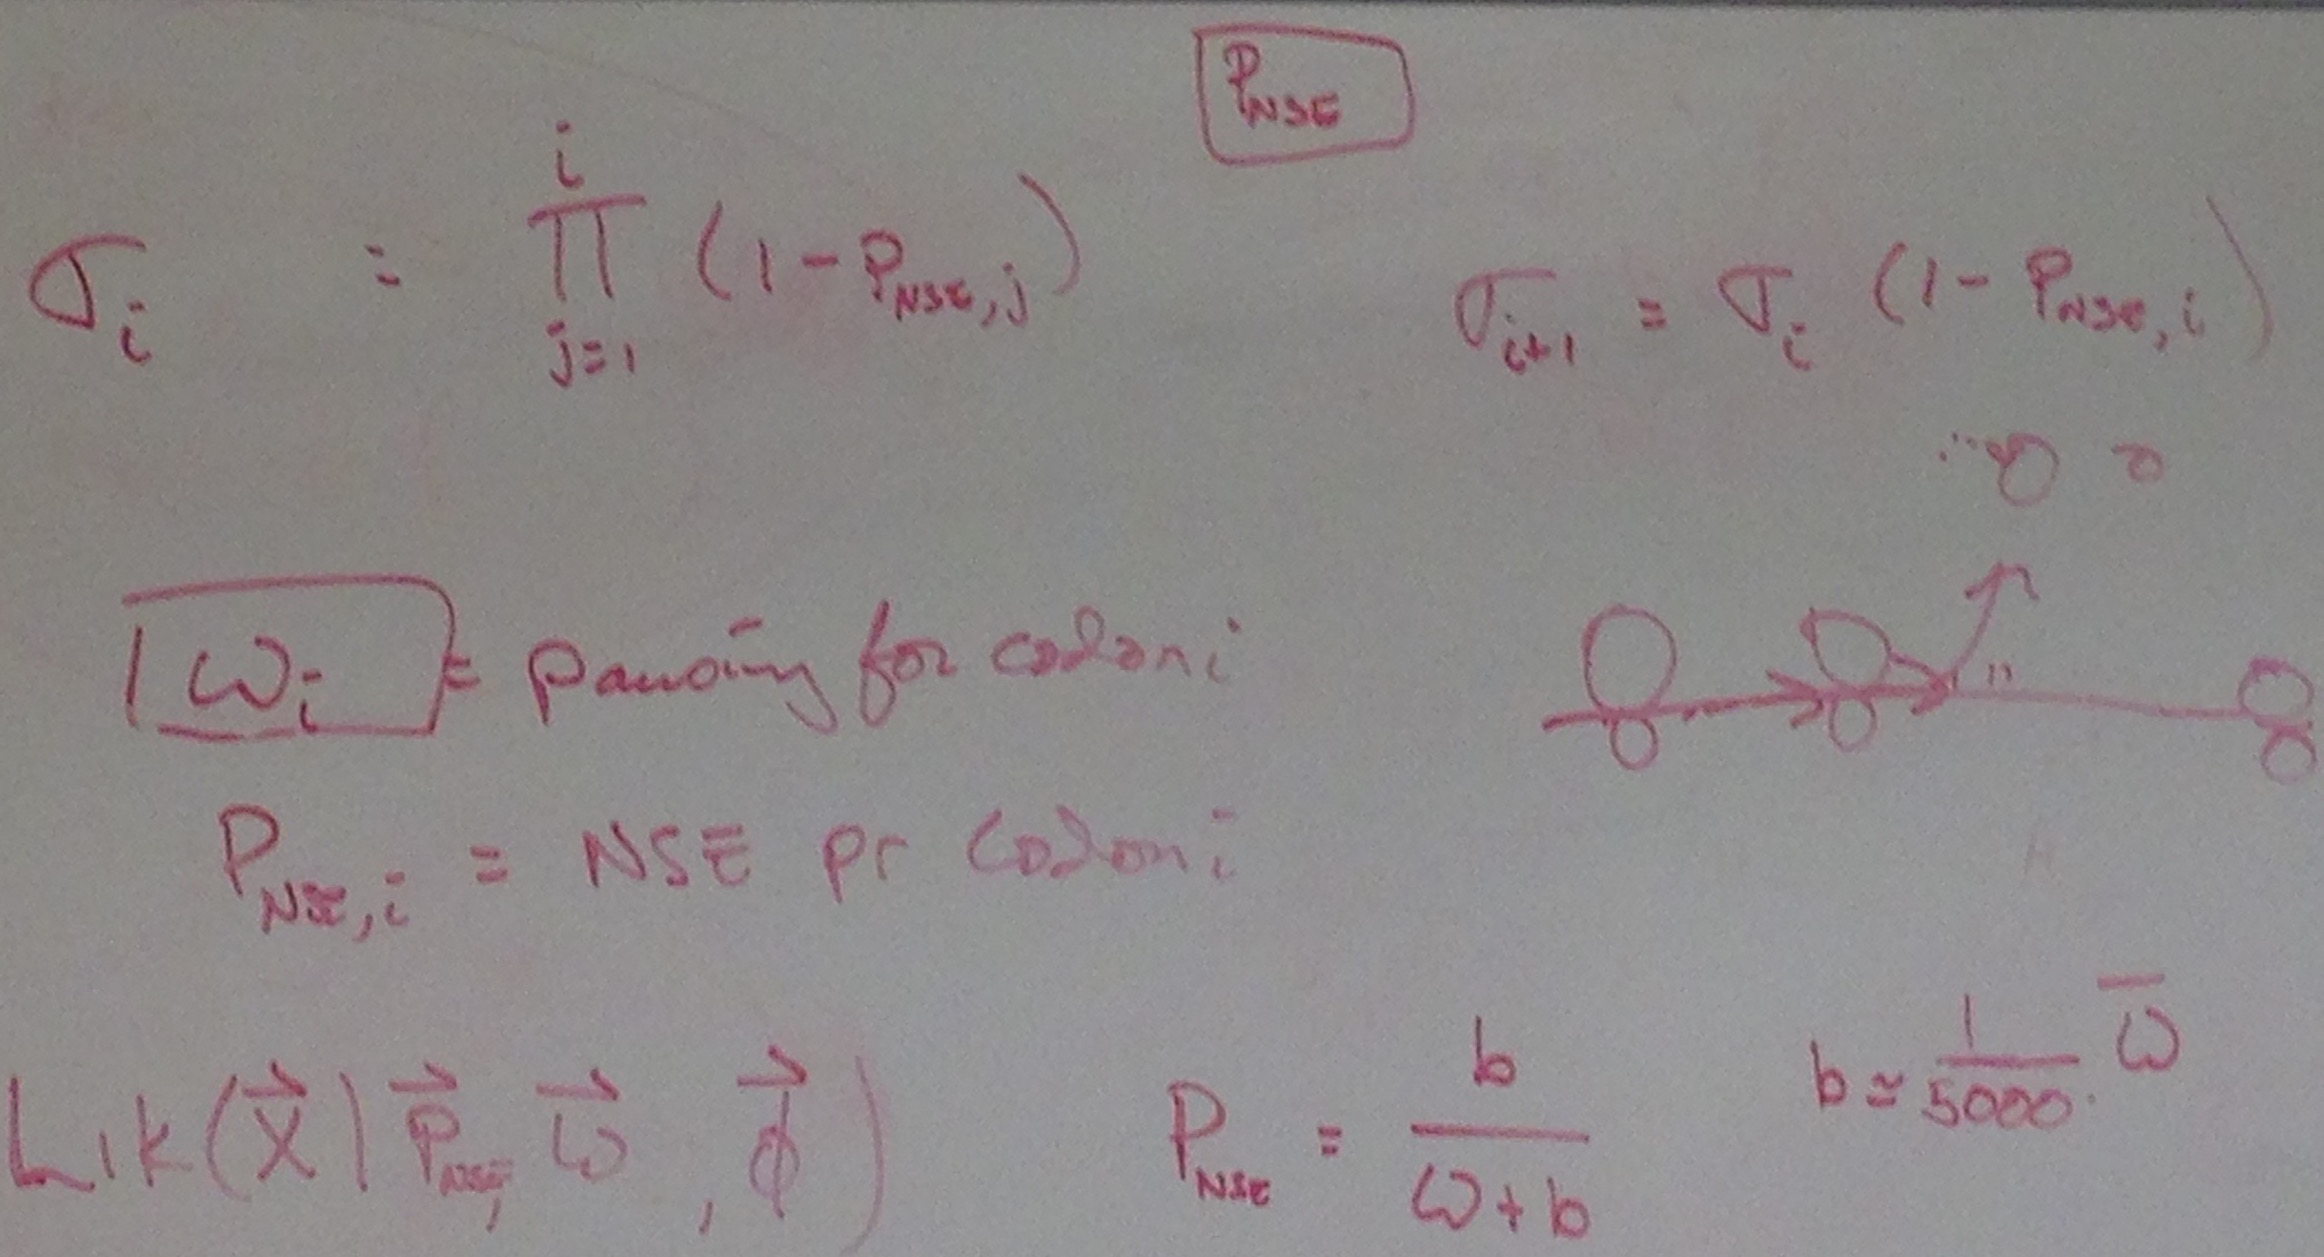
\includegraphics[width=\textwidth,keepaspectratio]{figures/5-13-16img.jpg}
    \label{PANSE Concept 5-13-16}
\end{figure}

\begin{equation}
    \sigma_{i} = \prod_{j=1}^{i} (1 - P_{NSE,j})
\end{equation}

$\omega_i$ = pausing for codon i

$p_nse, i$  = NSE $\Pr$ (probability) for codon i

This is codon-based.

Likelihood of the data given the parameters: 
$\mathcal{L}(\vec{x}|\vec{P_{NSE}},\vec{\omega}, \vec{\phi})$

Will be a much smaller data set, and with hundreds of calculations rather than thousands.

Randomly select $\sim$600 genes instead of 5400

Sigma vector of: $\sigma_{i + 1} = \sigma_i (1 - P_{NSE, i})$

Function is of probability of getting there vs waiting time once there

\experiment{TODOs}

\begin{itemize}
    \item Getting pausing values with simpler models (ROC)
    \item First analysis could be just estimating these terms
    \item This would mean creating a simulated data set.
    \item For simulation: $P_{NSE} = \frac{b}{\omega + b}$, where b is on the order of 1/5000 times average omega. ($b \simeq \frac{1}{5000}\overline{\omega}$) Talk to Jeremy about this, he may have finished this by now.
\end{itemize}

See the 2015 paper, 2011 paper with primal

\labday{May 19, 2016 Notes}

\experiment{PANSE Concepts}

rfp.model.pdf:
Reasoning [for lambda] is that for the sampling the Boltsman coefficient. See the explanation around equation (4) and the Z’s and Y’s.

Lambda Prime = Lambda.c * Z / Y, or call it K.

$\lambda^{\prime} = \lambda_c * \frac{Z}{Y}$

Z is the overall state space

Y is what is sampled

$\lambda_c = \lambda^{\prime} * \frac{C}{K}$. Let K be a new independent parameter, and keep track of Lambda Prime.

\labday{May 25, 2016 Notes}

\experiment{PANSE Concepts}

Codon-Specific Elongation Rate:
$P_{NSE} = \frac{b}{b + c}$ where b is where it flies off and c is where it continues.

Omega is the odds ratio of $\frac{P_{NSE}}{1 - P_{NSE}}$. Therefore $\omega = \frac{b}{c}$

Look at 2006, 2007 papers.

LOOK AT UPDATED PDF: IT’S IN FRAMEWORK

Psi (the symbol which I *thought* was Omega)
is the ribosome initiation rate: Rate at which ribosomes are jumping onto the mRA. Phi is the rate that they are jumping off at the very end.

If you have 50\% chance to get to the end, then Psi is twice as long as Phi

Phi = Psi * Sigma.

Don’t redo calculations from scratch, but rather in series.

\experiment{Parallelization}

\begin{itemize}
    \item Only 20 AA’s — Only 20 cores to spread load unto
    \item AA’s with 6 codons of course take more time than those with 2
\end{itemize}

Gilchrist thinks what is meant by Gene-Specific Parameters is to parallelize at the highest level, 
i.e. at the gene or amino acid level.

I should check the code; find where the OpenMP statements are, etc.

Mostly something to ask other people about if I want to tackle the problem.

\labday{May 26, 2016 Notes}

\experiment{Parallelization}

Cedric's input:
\begin{itemize}
    \item phi calculation, with MCMC accept/reject
    \item dynamic arrays
    \item big loop around everything
    \item code doesn’t work
    \item couldn’t figure out why
    \item didn’t spend that much time
\end{itemize}

we ended up parallelizing in the model class:

calculateLogLikelihoodRatioPerGene, apparently doesn’t do much.
Perhaps better to parallelize outside, with the big loop

Run a ROC model, then RFP

I’m running a fasta file that is simulated, so I know that it is true

I kinda need the R side

Get to the point where we suspect memory is the problem

Dynamic Arrays -\textgreater Vectors

\labday{May 31, 2016 Notes}

\begin{itemize}
    \item Start 1:21
    \item break 3:19
    \item back 3:24
    \item break 4:55
    \item return 5:02
    \item end 7:02
\end{itemize}

2 + 1.5 + 2

\experiment{Parallelization}

Go ahead and replace dynamic arrays with vectors, first

And then do this bare-bones calculation of runs to see if it makes it faster,
without regards to parallelization.

\labday{June 1, 2016 Notes}

\begin{itemize}
    \item Start 1:30
    \item Break 3:30
    \item Return 3:35
    \item End 7:00
\end{itemize}

2 + 3.5

\experiment{Parallelization}

From yesterday:

%\footnote{mikeg: June 18, 2016 - Please label your columns!
% Otherwise, it is impossible to know for certain what the data below represents.
%}
% Resolved June 27, 2016 (Hollis): Will do in the future, fixed it here as well

\begin{table}[H]
    \centering
    \begin{tabular}{|c|c|}
        \hline
        \textbf{Average Time with Dynamic Arrays} & \textbf{Number of Runs} \\
        \hline
        0.00621732 & 10 \\
        0.00687881 & 100 \\
        0.00947537 & 1000 \\
        0.00713974 & 10000 \\
        0.00785908 & 10000 \\
        0.00750889 & 10 \\
        \hline
    \end{tabular}
\end{table}

For today:

\begin{table}[H]
    \centering
    \begin{tabular}{|c|c|}
        \hline
        \textbf{Average Time with Vectors} & \textbf{Number of Runs} \\
        \hline
        0.0572747 & 10 \\
        0.0698414 & 100\\
        \hline
    \end{tabular}
\end{table}

…Odd, 10x as long on average

The above was in DEBUG mode. Release mode redos:

\begin{table}[H]
    \centering
    \begin{tabular}{|c|c|c|c|}
        \hline
        \textbf{A or V} & \textbf{Runs} & \textbf{Modifiers} & \textbf{Avg Time} \\
        \hline
        V & 100 & & 0.0141421 \\
        A & 100 & & 0.0047742 \\
        V & 10000 & & 0.00850093 \\
        A & 10000 & & 0.00479609 \\
        V & 10000 & No Deletion & 0.00871843 \\
        A & 10000 & No Deletion & 0.00491614 \\
        V & 10000 & std::sort & 0.00841396 \\
        \hline
        A & 10000 & & 0.00598796 \\
        A & 10000 & & 0.00520682 \\
        A & 100000 & & 0.00455916 \\
        A & 100000 & std::sort & 0.00776886 \\
        V & 100000 & & 0.00795495 \\
        V & 100000 & std::sort & 0.00785736 \\
        \hline
        A & 100000 & std::sort & 0.00383634 \\
        A & 100000 & & 0.00385638 \\
        A & 100000 & std::sort & 0.00392021 \\
        \hline
    \end{tabular}
\end{table}

Note: Vectors are ~2x as long on average now

\experiment{PANSE Implementation}

Next step: Make a list of everything PANSE touches and unit test these things (first and foremost before actually writing PANSE)

ALSO: Estimate and track how long, in reality, it takes to do each unit testing

PARFP, PTRFP? Just calling it RFP might be misleading.

\labday{June 2, 2016 Notes}

\begin{itemize}
    \item Start 1:01
    \item Break 3:35
    \item Return 3:50
    \item End 6:58
\end{itemize}

Spent till 4 (3 hours) compiling notes and creating a git directory.

\experiment{PANSE Implementation}

Expecting to spend ~1 hour deciding on what PANSE will need (or, rather, what RFP will need).

Talk with Gilchrist:

So data position feeds into:
\begin{itemize}
    \item a) data on gene 
    \begin{itemize}
        \item ab) to feed into ROC-RFP
    \end{itemize}
    \item or b) PANSE-RFP
\end{itemize}

\experiment{Lareau Data}
Which file type should I be reading in? RFP or Fasta?

For sample data for PANSE:

Lareau Paper -\textgreater GSE -\textgreater The untreated replicates 1,2,3. Take one, and even then only a subset of 
one of them as sample data.

The Lareau material may have undergone more processing that the new Weinberg GSE published Feb 10 2016. 

\enquote{Start with Lareau paper data} -- Gilchrist, 5:33

\labday{June 3, 2016 Notes}

\begin{itemize}
    \item Start 1:35
    \item Break 4:09
    \item Return 4:14 
\end{itemize}

\experiment{Lareau Data}

Decided to start reading the Lareau material. Began by looking directly at definition of data set
(I chose untreated replicate 1) and then parse the data to get a smaller subset (file size otherwise
is too large at 35MB)

Took longer than expected... When files finally parsed, 5:45.

Now have a data set of size 400 KB: those genes with 11 to 100 (inclusive) codons. 

\labday{June 6, 2016 Notes}

\experiment{TODOs}

Immediate future goals:
\begin{enumerate}
    \item Generate new Lareau material following specifications of Gilchrist talk, below.
    \item Just work, from now on, with the labbook class. Don't have to reformat old content.
    \item Formally write up a list of things TODO with Unit Testing for Parameter
    \item Unit Test up-to-date with Parameter
    \item Write up pseudo-code with PANSE itself to prepare for it
    \item Create and test a function for reading in Lareau material (low priority)
    \item Parallelization is after the initial PANSE stuff is implemented, very low priority
\end{enumerate}

\experiment{Lareau Data}

Talk with Gilchrist:

\begin{itemize}
    \item Let's get a randomly distributed set of data rather straight up isolation.
    \item See below for how to randomly distribute; want only 100 genes.
    \item 61 Parameters Pausing Time
    \item Lots of gene-specific parameters that scale with each gene.
    \item Let's say average of each gene is ~300 AAs.
    \item So ~7 observations per gene.
    \item 
    Try to get 2 parameters for a fair amount of information. 
    Calculating at sigma is going increase at gene length.
    \item And of course longer gene sequences take longer to parse.
    \item So probably want a data base for playing around with of 100 genes, between 200 and 400 AAs long
    \item Do we need to test with all 61 parameters?
    \item 2-codon AA's are the quickest thing to work with. 
    \item So may want to start with 100 genes of 200-400 AAs
    \item Estimate these parameters with a small subset of the codons, starting with the 2-codon ones.
    \item If they are behaving properly, scale up to 3/4/etc.
\end{itemize}

\noindent\makebox[\linewidth]{\rule{\paperwidth}{0.4pt}}

\begin{itemize}
    \item (Re: Lareau's distinction between long and short in the data)
    \item Long is de-facto standard
    \item Lareau argues that Short is also relevant despite usually being thrown out
    \item Long and short: tell how elongation is at each position.
    \item Our model is based on pausing. 
    \item So how do long and short factor in? Well, we don't know yet.
    \item We could base it on just one or the other or combine the two.
    \item For now let's just base it on Long.
\end{itemize}

\noindent\makebox[\linewidth]{\rule{\paperwidth}{0.4pt}}

After about thirty minutes following the talk with Gilchrist -- new 
subset of data produced via modifying old Perl scripts. Now have the specified data set
in the final \enquote{finalData.txt} -- 516 KB.

Interestingly small size -- seems like old data set had that many genes of smaller AA length.

\noindent\makebox[\linewidth]{\rule{\paperwidth}{0.4pt}}

Spent an hour afterward reading over labbook documentation and reformatting notes where needed.

\labday{June 7, 2016 Notes}
In the course of running an RFP Model, the following functions are called (and have yet to be
unit tested).

\experiment{TODOs}

\begin{itemize}
    \item initParameterSet (actually already done... mostly) -- general parameter
    \begin{itemize}
        \item test std\_csp changes -- Done
        \item test numAcceptForCodonSpecificParameters changes -- Done
        \item Possibly setNumMutationSelectionValues -- Ignore for now
        \item Possibly initCategoryDefinitions --Ignore for now
        \item For the two above -- Find how to check delM and delEta of category (a vector of Mixture Definitions) -- Done
        \item Check many final changes at the end of this function -- Three remaining
    \end{itemize}
    \item initRFPParameterSet -- RFP exclusive
    \item getSelectionCategory -- general parameter -- Done
    \item InitializeSynthesisRate -- general parameter
    \begin{itemize}
        \item calculateSCUO
        \item quickSortPair
        \item quickSort
        \item Parameter::randLogNorm
    \end{itemize}
    \item setParameter -- RFP model exclusive
    \item mcmc.run -- MCMC function on RFP(TODO later?)
\end{itemize}

\experiment{Unit Testing}

Going to take it one step at a time, finish up initParameterSet testing...

Finished most of initParameterSet completely. Need to ask Cedric about a duplicate function before
finishing the final two functions.

May need to write a function to unit test with the categories variable itself, but
all that happens otherwise is it pushes unto the vector of vector of vectors.

Encountering a strange printing bug right before the end. While if statement works correctly,
the final confirmation of initParameterSet isn't being printed.

Example output:

\noindent\begin{minipage}{\linewidth}
\begin{lstlisting}
Parameter getMixtureAssignment --- Pass
Parameter setMixtureAssignment --- Pass
Parameter getMutationSelectionState --- Pass
Parameter getNumParam --- Pass
Parameter getNumMixtureElements --- Pass
Parameter getStdDevSynthesisRate --- Pass
Parameter setStdDevSynthesisRate --- Pass
Parameter getCurrentStdDevSynthesisRateProposalWidth --- Pass
Parameter getNumAcceptForStdDevSynthesisRate --- Pass
Parameter getStdCspForIndex --- Pass
Parameter getNumAcceptForCspForIndex --- Pass
Parameter getNumMutationCategories --- Pass
Parameter getNumSelectionCategories --- Pass
Parameter getMutationCategory --- Pass
Parameter getSelectionCategory --- Pass
Parameter getMixtureElementsOfMutationCategory --- Pass
Parameter getMixtureElementsOfSelectionCategory --- Pass
Parameter getCategoryProbability --- Pass
Parameter setCategoryProbability --- Pass
Parameter getSynthesisRate --- Pass
Parameter setSynthesisRate --- Pass
Parameter getSynthesisRateProposalWidth --- Pass
0
Parameter initParameterSet --- Pass

Process finished with exit code 0
\end{lstlisting}
\end{minipage}

vs

\noindent\begin{minipage}{\linewidth}
\begin{lstlisting}
Parameter getMixtureAssignment --- Pass
Parameter setMixtureAssignment --- Pass
Parameter getMutationSelectionState --- Pass
Parameter getNumParam --- Pass
Parameter getNumMixtureElements --- Pass
Parameter getStdDevSynthesisRate --- Pass
Parameter setStdDevSynthesisRate --- Pass
Parameter getCurrentStdDevSynthesisRateProposalWidth --- Pass
Parameter getNumAcceptForStdDevSynthesisRate --- Pass
Parameter getStdCspForIndex --- Pass
Parameter getNumAcceptForCspForIndex --- Pass
Parameter getNumMutationCategories --- Pass
Parameter getNumSelectionCategories --- Pass
Parameter getMutationCategory --- Pass
Parameter getSelectionCategory --- Pass
Parameter getMixtureElementsOfMutationCategory --- Pass
Parameter getMixtureElementsOfSelectionCategory --- Pass
Parameter getCategoryProbability --- Pass
Parameter setCategoryProbability --- Pass
Parameter getSynthesisRate --- Pass
Parameter setSynthesisRate --- Pass
Parameter getSynthesisRateProposalWidth --- Pass


Process finished with exit code 0
\end{lstlisting}
\end{minipage}

\labday{June 8, 2016 Notes}

\experiment{Unit Testing}
%\footnote{mikeg: June 18, 2016 - Please use the `itemize' or `enumerate' environment for lists.
%  This helps keep things organized and easier to read.
%}
% Resolved June 27, 2016 (Hollis): Fixed this section, will keep in mind for the future.
\begin{itemize}
    \item Started by writing and testing a function for numAcceptForSynthesisRate.
    \item Printing this statement seems to have fixed the odd print bug mentioned yesterday.
    \item After doing that, I decided to write up on the documentation of Unit Testing I have done so far.
\end{itemize}

Asked Cedric re: get\sep Selection\sep Category and get\sep Synthesis\sep Rate\sep Category (paraphrased):

\begin{displayquote}
It's related to how we may have delta and Phi values...

We are trying to find out how efficient your codons have to be to reach a production rate
assuming cost is constant.

Cost = Benefit * production rate (Phi)

%\footnote{mikeg: June 18, 2016 - This is \emph{incorrect}. 
%  \begin{itemize} 
%  \item $\eta = $Cost\/Benefit 
%  \item Energy Flux to meet target production rate $\phi$ $= \eta * \phi$
%  \end{itemize}
%}
% Resolved June 27, 2016 (Hollis): These were roughly written notes as noted before.
% Commenting out to ensure that future readings don't mistake this as fact.

Switching to a different selection environment:
Different cost, different benefit, and therefore different Phi. \footnote{mikeg: June 18, 2016 
- Just to be clear, the likelihood of a given $\phi$ changes with changes in either 
\DeltaEta and\/or \DeltaM 
}

If you have 2 selection categories, you have to have two synthesis categories. 
They are the same even if we don't know them, but it saves renaming it to something more general.
\end{displayquote}

Finally finished initParameterSet besides checking categories matrix itself (minor, to do later).

Continued TODO:

\experiment{TODOs}

\begin{itemize}
    \item initRFPParameterSet -- RFP exclusive
    \item InitializeSynthesisRate -- general parameter
    \begin{itemize}
        \item calculateSCUO
        \item quickSortPair
        \item quickSort
        \item Parameter::randLogNorm
    \end{itemize}
    \item setParameter -- RFP model exclusive
    \item mcmc.run -- MCMC function on RFP(TODO later?)
\end{itemize}

Next goals: Do the internal functions for InitializeSynthesisRate related to quickSort.

Finish up InitializeSynthesisRate.

\labday {June 9, 2016 Notes}

Began by checking github; fixed semicolon error and confirmed package worked correctly.

\experiment{TODOs}

To truly finish testing InitializeSynthesisRate, we would need:

\begin{itemize}
    \item calculateSCUO
    \item Parameter::randLogNorm
    \item quickSortPair
    \begin{itemize}
        \item pivotPair
        \begin{itemize}
            \item swap (doubles)
        \end{itemize}
    \end{itemize}
    \item quickSort
    \begin{itemize}
        \item pivot
        \begin{itemize}
            \item swap (ints)
        \end{itemize}
    \end{itemize}
\end{itemize}

Ask Cedric if it'd be a good idea to just use std::sort instead of quickSort.

The quick sort algorithms are very math-intensive, so Unit Testing them may be lower priority.

For now, I am switching to unit testing RFP-exclusive functions.

\begin{itemize}
    \item initRFPParameterSet (in RFPParameter.cpp)
    \begin{itemize}
        \item check currentCodonSpecificParameter
        \item check proposedCodonSpecificParameter
        \item check lambdaValues (optional -- currently unused variable)
        \item check numParam -- Done
        \item check bias\_csp -- always set to 0, can ignore for now
        \item check std\_csp -- Done
        \item check groupList -- Done
    \end{itemize}
    \item setParameter (in RFPModel.cpp) -- may be untestable, ignore for now
\end{itemize}

In the course of working on checking RFPParameter, wrote up Unit Testing for all
Group List functions in Parameter.cpp

May need a wrapper function for current\sep Codon\sep Specific\sep Parameter and 
proposed\sep Codon\sep Specific\sep Parameter
extraction. Talk to Cedric.

Refocusing overall goals:
\begin{enumerate}
    \item Unit Test up-to-date with Parameter
    \begin{itemize}
        \item{initRFPParameterSet}
        \begin{itemize}
            \item check currentCodonSpecificParameter -- stalled, ask Cedric
            \item check proposedCodonSpecificParameter -- stalled, ask Cedric
        \end{itemize}
        \item{InitializeSynthesisRate}
        \begin{itemize}
            \item calculateSCUO
            \item Parameter::randLogNorm
            \item quickSortPair
            \begin{itemize}
                \item pivotPair
                \begin{itemize}
                    \item swap (doubles)
                \end{itemize}
            \end{itemize}
            \item quickSort
            \begin{itemize}
                \item pivot
                \begin{itemize}
                    \item swap (ints)
                \end{itemize}
            \end{itemize}
        \end{itemize}
        \item mcmc::run -- MCMC function on RFP
    \end{itemize}
    \item Write up pseudo-code with PANSE itself to prepare for it
    \item Create and test a function for reading in Lareau material (low priority)
    \item Parallelization is after the initial PANSE stuff is implemented, very low priority
\end{enumerate}

TODO tomorrow:

Ask about current/proposed CSP Parameter, quicksort vs std::sort, and how (if) to unit test
the more computation-intensive functions.

Finally replace cout statements in my own section of main.

Begin testing with MCMC run while waiting for others to arrive.

\labday {June 10, 2016 Notes}

There exists a hierarchy of functions to test before finally testing mcmc.run. Test the
subitems first: (NOTE: Testing with RFPModel)
\begin{itemize}
    \item mcmc::run
    \begin{itemize}
        \item mcmc::varyInitialConditions
        \begin{itemize}
            \item model::proposeCodonSpecificParameter -- wrapper to RFPparameter
            \item model::\sep propose\sep Hyper\sep Parameters -- wrapper to
            parameter::\sep propose\sep Std\sep Dev\sep Synthesis\sep Rate
            \item model::proposeSynthesisRateValues -- wrapper to parameter
            \item model::getGroupListSize -- wrapper to parameter (done?)
            \item model::getGrouping -- wrapper to parameter (done?)
            \item model::updateCodonSpecificParameter -- wrapper to RFPparameter
            \item model::\sep update\sep All\sep Hyper\sep Parameter -- 
            calls update\sep Std\sep Dev\sep Synthesis\sep Rate -- Ask
            \begin{itemize}
                \item updateStdDevSynthesisRate -- wrapper to parameter
            \end{itemize}
            \item model::getNumSynthesisRateCategories -- wrapper to parameter (done?)
            \item model::getSynthesisRateCategory -- wrapper to parameter (done?)
            \item model::getSynthesisRate -- wrapper to parameter (done?)
            \item model::getMixtureAssignment -- wrapper to parameter (done?)
            \item model::getStdDevSynthesisRate -- wrapper to parameter (done?)
            \item parameter::densityLogNorm
            \item paramter::randExp
            \item model::updateSynthesisRate -- wrapper to parameter
            \item model::updateGibbsSampledHyperParameters -- does not do anything
        \end{itemize}
        \item model::\sep set\sep Num\sep Phi\sep Groupings -- 
        a wrapper to parameter::\sep set\sep Num\sep Observed\sep Phi\sep Sets (done?)
        \item model::initTraces -- wrapper to RFPparameter initAllTraces
        \item model::updateTracesWithInitialValues
        \begin{itemize}
            \item parameter::updateSynthesisRateTrace
            \item parameter::updateMixtureAssignmentTrace
            \item RFPparameter::updateCodonSpecificParameterTrace
        \end{itemize}
        \item model::setLastInteration -- wrapper to parameter (done?)
        \item model::writeRestartFile -- wrapper to RFPparameter writeEntireRestartFile
        \item model::printHyperParameters -- unneeded to test, just prints
        \item model::getNumMixtureElements -- wrapper to parameter (done?)
        \item mcmc::acceptRejectCodonSpecificParameter
        \begin{itemize}
            \item model::calculateLogLikelihoodRatioPerGroupingPerCategory
            \item model::updateCodonSpecificParameterTrace
        \end{itemize}
        \item model::\sep adapt\sep Codon\sep Specific\sep Parameter\sep Proposal\sep Width 
        -- wraps RFP\sep parameter
        \item mcmc::acceptRejectHyperParameter
        \begin{itemize}
            \item model::calculateLogLikelihodRatioForHyperParameters
            \item model::updateHyperParameter -- parameter::updateStdDevSynthesisRate
            \item model::updateHyperParameterTraces
        \end{itemize}
        \item model::\sep adapt\sep Hyper\sep Parameter\sep Proposal\sep Widths -- 
        will call the function adapt\sep Std\sep Dev\sep Synthesis\sep Proposal\sep Width, 
        a wrapper to parameter. Uses traces.
        \item mcmc::acceptRejectSynthesisRateLevelForAllGenes
        \begin{itemize}
            \item model::\sep get\sep Mixture\sep Elements\sep Of\sep Selection\sep Category 
            -- wrapper to parameter (done?)
            \item model::calculateLogLikelihoodRatioPerGene
            \item model::getCategoryProbability -- wrapper to parameter (done?)
            \item parameter::randMultinom
            \item model::setMixtureAssignment -- wrapper to parameter (done?)
            \item model::updateSynthesisRateTrace
            \item model::updateMixtureAssignmentTrace
            \item model::calculateAllPriors -- currently does nothing
            \item parameter::randDirichlet
            \item model::setCategoryProbability -- wrapper to parameter (done?)
            \item model::updateMixtureProbabilitiesTrace
        \end{itemize}
        \item model::adaptSynthesisRateProposalWidth -- wrapper to parameter
        \item mcmc::calculateGewekeScore
    \end{itemize}
\end{itemize}

TODO:

Ask about why it is that Hyper Parameters == StdDevSynthesisRate, always

Don't know if we need to test wrapper functions i.e. those in Model that simply perform
a function in its associated Parameter object.

Ask about why dynamic arrays were in code in the first place, i.e. in randMultinom.

New modified list stripping out some things that are more-or-less done
(Or those that depend on unimplemented functions or those with random variables):
\begin{itemize}
    \item mcmc::run
    \begin{itemize}
        \item mcmc::varyInitialConditions
        \item model::initTraces -- wrapper to RFPparameter initAllTraces
        \item model::updateTracesWithInitialValues
        \begin{itemize}
            \item parameter::updateMixtureAssignmentTrace
            \item RFPparameter::updateCodonSpecificParameterTrace
        \end{itemize}
        \item model::writeRestartFile -- wrapper to RFPparameter writeEntireRestartFile
        \begin{itemize}
            \item parameter::writeBasicRestartFile
            \item writeRFPRestartFile
        \end{itemize}
        \item mcmc::acceptRejectCodonSpecificParameter
        \begin{itemize}
            \item model::calculateLogLikelihoodRatioPerGroupingPerCategory
            \item model::updateCodonSpecificParameterTrace
        \end{itemize}
        \item model::\sep adapt\sep Codon\sep Specific\sep Parameter\sep Proposal\sep Width --
        wraps RFP\sep parameter. Uses traces.
        \item mcmc::acceptRejectHyperParameter
        \begin{itemize}
            \item model::calculateLogLikelihodRatioForHyperParameters
            \item model::updateHyperParameter -- parameter::updateStdDevSynthesisRate
            \item model::updateHyperParameterTraces
        \end{itemize}
        \item model::\sep adapt\sep Hyper\sep Parameter\sep Proposal\sep Widths -- 
        will call the function adapt\sep Std\sep Dev\sep Synthesis\sep Proposal\sep Width,
        a wrapper to parameter. Uses traces.
        \item mcmc::acceptRejectSynthesisRateLevelForAllGenes
        \begin{itemize}
            \item model::calculateLogLikelihoodRatioPerGene
            \item model::updateSynthesisRateTrace
            \item model::updateMixtureAssignmentTrace
            \item model::updateMixtureProbabilitiesTrace
        \end{itemize}
        \item model::\sep adapt\sep Synthesis\sep Rate\sep Proposal\sep Width -- 
        wraps parameter. Uses traces.
        \item mcmc::calculateGewekeScore
    \end{itemize}
\end{itemize}

After writing the setNumObservedPhiGroupings and lastIteration unit testing functions and
updating these notes, worked on restart file writing.

TODO: Discuss with Cedric how to proceed to unit testing with restart files
in the future, i.e. keep in same function or separate.

Next step:

Probably work with traces. Not sure how to proceed with unit testing
the most complicated functions re: computation, nor with reading/writing files yet.

\labday {June 11, 2016 Notes}
Mostly read documentation. Worked from home, so no benefit of discussing implementation topics.
Worked less than planned.

\labday {June 13, 2016 Notes}
Discussing Unit Testing with Cedric:

OK'd changing quicksort (simple implementation) to std::sort.

Instead of running the higher-level functions that are directly used, 
probably better to stick to the simple functions and then test MCMC algorithm runs with
100 samples; compare the likelihoods of each model, which should be similar, to detect errors.

For the intense calculations, for now ignore. The calculation unit tests will be summed up (in a
general sense) by just doing MCMC algorithm runs.

First, going to change std::sort.

After that was done, decided to clean up some R-side unit testing in preparation of testing
MCMC algorithm runs -- since in R you can set seed for entire C-side implementation.

\experiment{TODOs}
\begin{itemize}
    \item Fix the TODO note in Parameter.cpp under initParameterSet 
    %\footnote{mikeg: June 18, 2006 - It is unclear what note you're referring to.
    % Recommend using \\label\{\} to label earlier note and \\ref\{\} command here to link to it.
    %  }
    % Resolved June 27, 2016 (Hollis): Will keep in mind in the future. Code in question
    % (current version, so changes already made):
    %
    %   for (unsigned i = 0u; i < numGenes; i++)
    %   {
    %       // Note: This section of code is because vectors in R are 1-indexed (i.e. for mixtureAssignment)
    %       //TODO:need to check index are correct, consecutive, and don't exceed numMixtures
    %       //possibly just use a set?
    %   #ifndef STANDALONE
    %       mixtureAssignment[i] = geneAssignment[i] - 1;
    %       //mixtureAssignment[i + 1] = geneAssignment[i];
    %%%%%%%%% Code is here, solved by Cedric ^ %%%%%%%%
    %   #else
    %       mixtureAssignment[i] = geneAssignment[i];
    %   #endif
    %   }
    \item Ask Cedric about:
    \begin{itemize}
        \item Testing restart files: keep in same function or separate unit tests.
        \item May need wrapper function for current\sep Codon\sep Specific\sep Parameter 
        and proposed\sep Codon\sep Specific\sep Parameter extraction. 
        \item How to actually run R-side scripts; weird error messages.
        \item What is the inst folder? Can we remove it, since it seems to be old Unit Testing Data stuff?
    \end{itemize}
\end{itemize}

Still need to look at Trace stuff as next major step without help from Cedric.

Spend at most two more days on Unit Testing at this rate; after, will start thinking solely
on PANSE.

\labday {June 14, 2016 Notes}

Yesterday ended by running memory leak checks in the background on a whim due to debugging
some new calls without associated delete calls.

Found a confirmed memory leak with my\_print. Started today by flushing output on
both C and R side of code, as well as expanding unit testing for Utility.h.

Spent an hour and a half on this.

Came in late, could not ask Cedric questions.

\experiment{Traces}
Order of Trace functions to examine in a typical model run (via MCMC::run):
\begin{itemize}
    \item model::initTraces(samples + 1, genome.getGenomeSize());
    \begin{itemize}
        \item RFPparameter-\textgreater initAllTraces
        \begin{itemize}
            \item traces.initializeRFPTrace (RFP-only)
            \begin{itemize}
                \item initializeSharedTraces
                \item initCodonSpecificParameterTrace (for both alp and lmPri)
            \end{itemize}
        \end{itemize}
    \end{itemize}
    \item model::updateTracesWithInitialValues(genome) -- TO BE EXAMINED
    \begin{itemize}
        \item parameter::updateSynthesisRateTrace
        \begin{itemize}
            \item traces.updateSynthesisRateTrace
        \end{itemize}
        \item parameter::updateMixtureAssignmentTrace
        \begin{itemize}
            \item traces.updateMixtureAssignmentTrace
        \end{itemize}
        \item RFPparameter::updateCodonSpecificParameterTrace
        \begin{itemize}
            \item traces.updateCodonSpecificParameterTraceForCodon (for alp and lmPri)
        \end{itemize}
    \end{itemize}
    \item mcmc::acceptRejectCodonSpecificParameter
    \begin{itemize}
        \item model::calculateLogLikelihoodRatioPerGroupingPerCategory
        \item model::updateCodonSpecificParameter(grouping)
        \item model::updateCodonSpecificParameterTrace
    \end{itemize}
    \item model::\sep adapt\sep Codon\sep Specific\sep Proposal\sep Width -- 
    wrapper to RFP\sep parameter. Uses trace
    \item mcmc::acceptRejectHyperParameter
    \begin{itemize}
        \item model::calculateLoglIkelihoodRatioForHyperParameters
        \item model::updateHyperParameter - parameter::updateStdDevSynthesisRate
        \item model::updateHyperParameterTraces
    \end{itemize}
    \item model::\sep adapt\sep Hyper\sep Parameter\sep Proposal\sep Widths -- 
    will call the function adapt\sep Std\sep Dev\sep Synthesis\sep Proposal\sep Width,
    a wrapper to parameter. Uses traces.
    \item mcmc:acceptRejectSynthesisRateLevelForAllGenes
    \begin{itemize}
        \item model::calculateLogLikelihoodRatioPerGene
        \item model::updateSynthesisRateTrace
        \item model::updateMixtureAssignmentTrace
        \item model::updateMixtureProbabilitiesTrace
    \end{itemize}
    \item model::adaptSynthesisRateProposalWidth -- wrapper to parameter. Uses traces.
\end{itemize}

This list is still incomplete, but we shall start implementing now for convenience.

Need to keep examining functions... 

Ended before checking model::updateTracesWithInitialValues

\labday {June 15, 2016 Notes}

Answers to Cedric questions:
\begin{itemize}
    \item In general, design of code is up to me. Seems good with whatever.
    %\footnote{mikeg: June 18, 2016 - This seems like a poor idea and more guidance for code design should be provided given the fact that many folks work on this code.
    %}
    % Resolved June 27, 2016 (Hollis): Agree with mikeg. Since this comment Cedric has
    % created a general formatting document, and I will merge my unofficial one that I
    % had been working on with his once I discuss it.
    \item DevRScripts are super outdated. Be careful of what to use, i.e. a lot of functions
    are using old definitions and need additional arguments.
    \item Again, for overall unit testing:
    \begin{itemize}
        \item Do a run, know what the output is.
        \item 
        Then repeat that run in the testThat function, compare the two runs. As long as outputs are the same, everything is fine.
    \end{itemize}
    \item Good scripts to base code off of: all\sep Unique scripts.
    Mainly all\sep Unique\sep \_\sep kl\sep \_\sep reduced.R, 
    all\sep Unique\sep \_\sep sim\sep Mod.R
    \item Bad script: runROCModelFromGoodValues.R
\end{itemize}

Cedric commented that there was a lot of old and outdated files, so I spent some time
trying to clean up the more obvious files.

\begin{itemize}
    \item Removed inst folder from RibModelFramework.
    \item Removed cleanSeq() finally
    \item Cut down on number of my\_print calls; hopefully increases efficiency slightly
    in either compilation of running phase.
\end{itemize}

Afterward attempted to learn more about R in order to write scripts to test models with set\_seed.

Testing Restart files:

I think I will create a separate function for each type of file. Basic Parameter, RFP, ROC, etc.

These will be tested by first checking if both read and write work at the same time.

For basic parameter checking, for example, perhaps 1) use initParameter manually, like before.

2) Then write the file

3) Then read in the file and compare with established, manually set variables.

\experiment{TODOs}

For tomorrow:

Unit Test with Restart files. This will help confirm any results.

Continue working with R model unit testing

Cedric will likely not be in for the rest of the week; will continue jumping around with
work assignments until after my vacation period.

\labday {June 16, 2016 Notes}

\experiment{R Debugging}
Began the day immediately encountering completely unknown errors attempting to run any
R scripts that had worked the day before. Problem seems to be with MCMC\_run. As Cedric
is not here today, will be much more difficult to check R-side scripts. At the same time,
worry that any changes made today may mess up the project as a whole despite
the Travis check declaring no errors. Will probably not push any changes made today
unless I can debug this.

Decided to clean up the mess of warnings spat out in order to find out how to debug:
I changed the deprecated Rcpp::\sep load\sep Rcpp\sep Modules() function
to several Rcpp::\sep load\sep Module() functions, 
leaving a comment to discuss this change in the future with Cedric

Then, I minorly edited the documentation files to clear up the more obvious errors.

\labday {June 17, 2016 Notes}

\experiment{R Debugging}
Continued working on fixing R documentation.

Finishing at 6 after about 4 hours of work and research, I was able to reduce the warnings
on my own machine to 4 Warnings and 2 Notes.

The unknown errors and R studio crashing thing has been fixed, but I'm not sure how.
I suspect it may have been errors in building/installing the package, but I checked out
a fresh copy of all of the files.

Goals for next work days: Restart file testing, model testing, PANSE pseudocode.

Will probably switch to PANSE pseudocode over the vacation period if I have any time to work,
so I can discuss any ideas I may have with Dr. Gilchrist once he returns.

\labday {June 27, 2016 Notes}

\experiment{R Debugging}

\begin{itemize}
\item 
Last night (June 26) spent about two hours fixing a bug with the overall project:
there was an error with testhat due to changing (fixing) Parameter.cpp setup.
\item
Plan for today is to begin unit testing with R-side models while also rereading PANSE
documentation and planning psuedocode.
\item
Found a bug in function to simplify code; fixed bug, started replacing this code
in the existing R scripts for consistency. 
Took an hour and a half.\footnote{mikeg: 06/30/16 -- You should state more clearly what this bug so that if you needed to go back and remember what you did, you'd be able to do so from your notes.
You spent 1.5 hours fixing this bug, why not spend a few more minutes documenting the problem and fix?}
\footnote{mikeg: 06/30/16 -- Also, instead of commenting out the footnotes and then responding to them, instead add a new line to the footnote and put your reponse there.
That way I can go through them and comment them out if I feel they are resolved.
} 
\footnote{Hollis: 07/05/16 -- Acknowledged. 
I don't know if you want me to un-comment-out the old footnotes, but I will not do this in the future.
The bug mentioned was in R/parameterObject.R: two functions (getMixtureAssignmentEstimate and getExpressionEstimatesForMixture) did not apply the unlist function for a random of values, and it has been corrected now.}
\item
Fixed another bug with traces on the R-side whenever plotting is done.\footnote{mikeg: 06/30/16 -- Better than the above note, but could still use a little more detail.}
\footnote{Hollis: 07/05/16 -- Acknowledged. 
Bug was in R/plotParameterObject.R, where a function re-set the samples to 100 no matter what the actual argument was (now fixed).}
\end{itemize}

Talk with Dr. Gilchrist:

\begin{itemize}
    \item Use our simulated results getting pausing time
    (but with almost no or no nonsense error) and compare to published results.
    \item Accuracy— within 80-90\% close estimates. Look at Laraeu data or Weinberg
    \item Plot our estimates vs their estimates and hope to see a nice regression.
    \item Also compare the deltaEta values from the 2015.
    \item Pausing times are the inverse of the rates.
    \item 3 places to find data:
    \begin{itemize}
        \item Lareau et al
        \item 
        Pop et al -- Main focus. Check Gauley: highest-level directory -\textgreater tmp -\textgreater Pop...
        Also ghanas's documents are now open. Gabriel worked with some of this data before but it
        is undocumented, so just restart from scratch.
        \item Weinberg et al
    \end{itemize}
\end{itemize}

Spent a bit of time cleaning up notes afterward. Will clean up further at home.

Also, some Cedric answers:
\begin{itemize}
    \item 
    I can go ahead and publish the unofficial style changes I had been working on on the side
    Cedric can just review them later.
    \item
    To debug the current unknown error with Rstudio and allUnique\_simMod.R, I should
    go line-by-line and execute. 
    The problem seems to be with \enquote{plot(model, genome, parameter, samples = samples*0.1, mixture = mixture, main = Codon Usage Plot)}.
\end{itemize}

\labday {June 28, 2016 Notes}

Did not end up having time to clean up at home, began cleaning up notes today instead.\footnote{mikeg: 06/30/16 -- As previously requested, please use the itemize environment when listing stuff. 
}
\footnote{Hollis: 07/05/16 -- Acknowledged. This small section of text had slipped through the cracks, and the rest of the text has itemize used.}

Finished after an hour of commenting, then decided to integrate my unofficial style guide
into the one Cedric had created.

Spend about 45 minutes on this before pushing changes. Going to now debug the R code error(s).

\experiment {R Debugging}

Cedric helped me with finding a minor and easy-to-fix bug where a redefined function
now has an extra argument, which is now properly accounted for on the R-side of the code.\footnote{mikeg: 06/30/16 -- Ibid}
\footnote{mikeg: 06/30/16 -- I would appreciate it if, when working with LaTeX, you did not have your editor break the lines at a fixed width.
Instead, I recommend you put a each sentence on a separate line.
}
\footnote{Hollis: 07/05/16 -- Acknowledged.
I am not sure what you mean by Ibid.}

However, I have now encounted a much more difficult bug to trace back its origins:\footnote{mikeg: 06/30/16 -- Why are you using \emph{minipage} below?
Also, the code failed to show up when I used pdflatex wether I used the minipage environment or not. 
Please confirm it shows up when you latex it.
\label{fn:lstError}
}
\footnote{Hollis: 07/05/16 -- it seems like the latex version of my notes I had uploaded last was in draft mode, defined at the top, which I use to see errors more easily.
I will try to keep it in release mode in the future (which does show minipages etc.).}

\noindent\begin{minipage}{\linewidth}
\begin{lstlisting}
for (aa in names.aa) 
{ 
    if (aa == "M" || aa == "W" || aa == "X") next 
    codons <- AAToCodon(aa, T) 
    for (i in 1:length(codons)) 
    {
        selection <- c(selection, parameter$getCodonSpecificPosteriorMean(mixture, samples*0.1, codons[i], 1, T)) 
        selection.ci <- c(selection.ci, parameter$getCodonSpecificVariance(mixture, samples*0.1, codons[i], 1, TRUE, T)) 
        mutation <- c(mutation, parameter$getCodonSpecificPosteriorMean(mixture, samples*0.1, codons[i], 0, T)) 
        mutation.ci <- c(mutation.ci, parameter$getCodonSpecificVariance(mixture, samples*0.1, codons[i], 0, TRUE, T)) 
    } 
} 
\end{lstlisting}
\end{minipage}


It seems that the function call 
\enquote{parameter\sep \$get\sep Codon\sep Specific\sep Variance\sep (mixture, samples*0.1, codons[i], 1, TRUE, T)} is not working.

This function returns the value NaN, which is then continually combined into an array of NaNs 
which results in a later call of setting the standard deviation to have \enquote{incorrect number
of dimensions}.

From its exposure to RCPP, this function is tracked to a function defined in the R section of
Parameter.cpp, and from there it uses a C-side function that involves a lot of calculations.

I decided to check this by putting in many temporary print statements 
to track the variables; it seems
the normalizationTerm somehow becomes infinity if this function is used with
10 samples (which becomes only 1) and it is unbiased: the normalizationTerm
is calculated as \verb+(1 / (samples - 1.0))+ in this case.\footnote{mikeg: 06/30/16 -- Do you mean 10 samples or 10 steps of the MCMC?  
I expect it is the latter.
Is this function related to calculating a variance? (this makes sense in the context and the fact you talk about biased and unbiased).
In general, you want to have at least 3 samples when calculating a variance or variance.
If you have only 1, then you're in trouble and this may explain why the error that persists.
I would argue the code should test the sample size and if it's below the necessary number, such as 3 for calculating the variance, the code either exits telling the user to increase their sample size or, depending on what exactly being calculated and what it's being used for, a Warning thrown and a default value used.
}
\footnote{Hollis: 07/05/16 -- It happens with 10 samples. 
And yes, it works with variance.
I understand why the bug occurs, which is why we ended up implementing the solution we did.
Is 3 an optimal number?
I believe Cedric and I had decided to just account for this worst-case by making the sample size only 1 throw an error, but it is easily changed and very justifiable to have the minimum be higher.
Currently, we do not exit -- we throw a Warning and instead of making it unbiased, we make it biased.
This does mean we do not change the number of samples that are used.}

Asked Cedric for input; I believe this might be a case we have to account for.

Added the case with a warning that forced it be to biased rather than unbiased.

However, the dimension error still exists; it must have been a separate issue I fixed.

Will have to ask Cedric again tomorrow.

Possible next course of action: figure out why there is another invalid method
in run\sep Simulated\sep RFP\sep Data\sep .\sep R in Rib\sep Model\sep Dev:
\footnote{mikeg: 06/30/16 -- same as footnote \ref{fn:lstError}}
\footnote{Hollis: 07/01/16 -- See answer on \ref{fn:lstError}}
\footnote{mikeg: 06/30/16 -- Is the lstlisting for code or output or both?}
\footnote{Hollis: 07/01/16 -- This is the part of the code in runSimulatedRFPData.R that causes an error.
Technically, it is both code and output since it was run with Rstudio (which prints and runs the code and then any outputs/errors as well).}

\noindent\begin{minipage}{\linewidth}
\begin{lstlisting}
> for (i in 1:61)
+ {mikeg: 06/30/16 --
+ codon <- codonList[i]
+ alphaList[i] <- parameter$getCodonSpecificPosteriorMean(cat, samples * 0.5, codon, 0, F)
+ alphaTrace <- trace$getCodonSpecificParameterTraceByMixtureElementForCodon(1, codon, 0)
+ alpha.ci[i,] <- quantile(alphaTrace[(samples * 0.5):samples], probs = c(0.025,0.975))
+ lambdaPrimeList[i] <- parameter$getCodonSpecificPosteriorMean(cat, samples * 0.5, codon, 1, F)
+ lambdaPrimeTrace <- trace$getCodonSpecificParameterTraceByMixtureElementForCodon(1, codon, 1)
+ lambdaPrime.ci[i,] <- quantile(lambdaPrimeTrace[(samples * 0.5):samples], probs = c(0.025,0.975))
+ waitingTimes[i] <- alphaList[i] * lambdaPrimeList[i]
+ }
Error: could not find valid method
\end{lstlisting}
\end{minipage}

Until I can confidently run a script at all in R I don't feel confident testing on R --
prone to errors before I can even run unit testing, currently.\footnote{mikeg: 06/30/16 -- This doesn't make any sense to me.  Please try to be clearer in your notes. }
\footnote{Hollis: 07/05/16 -- Acknowledged. 
I was basically making a note to myself that I should work on making any given script run in R since I was encountering a hodgepodge of errors before I even try to run unit testing.}

\labday {June 29, 2016 Notes}

Began by asking Cedric re: the script all\sep Unique\sep \_\sep sim.R, and fixed the dimension bug.\footnote{mikeg: 06/30/16 -- Please document the nature of the bug and the fix!}
\footnote{Hollis: 07/05/16 -- This bug was likely caused by the old developmental scripts not being updated in general.
It seems that a function (upper.panel.plot) that used to accept a normal distribution's standard deviation, manually calculated, now accepts any standard deviation in the form of a matrix: this matrix will contain the upper and lower standard devation thresholds.
To fix the bug, I copied code from getCSPEstimates.Rcpp\_ROCParameter in R/parameterObject.R which creates a standard deviation matrix in an almost identical way to what the script would want.\label{fn:dimensionFix}}

Used a different function and rendered results as a matrix, can now produce correct .pdf files.
\footnote{mikeg: 06/30/16 -- Which function? Why?  
Don't expect to remember these details.  
Document them!
}
\footnote{Hollis: 07/05/16 -- See other footnote, \ref{fn:dimensionFix}.}

Then fixed run\sep Simulated\sep RFP\sep Data.R: invalid method occurs calling:
\enquote{alpha\sep Trace \sep \textless-\sep trace\sep 
\$\sep get\sep Codon\sep Specific\sep Parameter\sep 
Trace\sep By\sep Mixture\sep Element\sep For\sep Codon\sep (1\sep,\sep codon\sep,\sep 0)}

Fixed the error occurring early, which was another missing argument due to the script being old.

With this done, began setting up things on Gauley again:
\begin{itemize}
    \item Created and updated the RibModel repos.
    \begin{itemize}
        \item TODO: Set up SSH key and passphrase
    \end{itemize}
    \item Moved the pop et all data to my home directory on Gauley and locally.
\end{itemize}

I spent some time reorganizing materials so I know where everything is:

\begin{itemize}
    \item Weinberg Data
    \begin{itemize}
        \item Found in an email sent by Dr. Gilchrist April 15, 2016.
        \item Paper link: \url{http://biorxiv.org/content/early/2015/07/06/021501}.
        \item Materials and Locations:
        \begin{itemize}
            \item gilchrist-notes/Apr22-premal
            \begin{itemize}
                \item email.premal.07.21.2015.txt
                \item GSE53313\_readMe.txt
                \item WeinbergMain.pdf
                \item WeinbergSupplemental.pdf
                \item GSM1969533\_Unselected\_RPKMs.txt -- 
                retrieved from paper's supplemental information link.
            \end{itemize}
            \item gilchrist-lfs/Apr22-premal: RPF\_read\_positions.GSE3313.txt.gz
            (the extracted file is renamed data.txt)
        \end{itemize}
    \end{itemize}
    \item Lareau Data
    \begin{itemize}
        \item Paper link: \url{https://elifesciences.org/content/3/e01257}.
        \item PDF found as LareauMain.pdf in gilchrist-notes/lareau.
        \item GSM1406463\_untreated\_1.percodon.txt --
        retrieved from paper's supplemental information link. In gilchrist-lfs/lareau.
    \end{itemize}
    \item Pop Data
    \begin{itemize}
        \item Paper link: \url{http://www.ncbi.nlm.nih.gov/pmc/articles/PMC4300493/}.
        \item Huge directory containing most of the content of the article, including supplementary notes, figures, and some data is found in gilchrist-lfs/Pop.
        \item Some work had been done on Pop already when Gabriel was on the team (April 26) -- see the rfpSort directory, now under gilchrist-notes/Pop.
        \item Further work on redoing and documenting analysis is being done in gilchrist-notes/Pop/rfpProcessJuly6
        \item rfp\sep .\sep count\sep .\sep data\sep .\sep by\sep .\sep gene\sep .\sep codon\sep .\sep and\sep .\sep position\sep .\sep GSE63789\sep .\sep wt\sep .\sep csv
        \item This file is from an unknown source; located in gilchrist-notes/Pop/rfpSort.
    \end{itemize}
\end{itemize}

\labday {June 30, 2016}

Began to write scripts to running and testing models.

Starting with the ROC model because the working script I had been debugging is based on that.

Goals:

\begin{itemize}
    \item Modify existing script into a unit testing script.
    \item Compare the simulated data with any results I can find in the papers organized yesterday.
    \item Automate this check and incorporate it into the main package.
\end{itemize}

\begin{itemize}
    \item Started by noticing a operating system independent function for grabbing file locations.
    Will talk to Cedric (who is not in today) to add this into mainline code.
    \item Also need to ask him about running things remotely on Gauley.
    Alan has been using the computer directly to run R studio and get plots etc., and it'd be inconvenient if we have to share in the future.
    \item Since this is the case, I can probably shelf the github passphrase thing until a more
appropriate time.
    \item Changed occurrences of \verb+paste+ to \verb+paste0+ in the package's R code -- slightly
more efficient implementation without separators.
    \item Looks like the script I wrote works based on its modified file location. 
    What remains is to have a concrete result to compare it to (currently don't know what to look for).
    \item Started by reading the Pop 2014 paper.
\end{itemize}

Talked with Dr. Gilchrist further --

\begin{itemize}
    \item Again, we are working with RFP data rather than fasta data. Seems like all
    the data I have available to me is for RFP rather than ROC-based.
    \begin{itemize}
        \item On that note, strongly consider talking to Cedric about renaming our models in
        the code. The distinction between RFP ROC and "regular ROC" isn't very clear right now.
    \end{itemize}
    \item With this in mind, stopping work on the ROC model file I have been editing.
    Nice as reference for future code but continuing to think of outputs in this form
    detracts from my understanding of what we're doing in the big picture.
    \item Instead, recall the supplemental material descriptions of what is in the Pop folder
    I have extracted. It will describe better what they get: in particular, look at Codon
    Translation Rates (codon.specific.translation.rates.table.xlsx) for rates.
    \item Recall that in the Pausing Time Definition, we \textbf{do} get pausing times.
    \item As mentioned before, these pausing times are the inverse of the translation rates.
    \item The pausing time model (RFP) does get the Lambda and Alpha values.
    \item The paper defines the estimated waiting time as alpha over lambda.
    \item So we can plot these estimated waiting times to 1 over the translation rates
    (or vice-versa) to determine if they all line up -- that the unknown factor times the
    elongation-based translation rate in the Pop paper is equivalent.
    \item TODO: Document this way better than currently, once this has been implemented.
    \item TODO: Grab the data and feed it into our model for simulation: GSE63789\sep \_\sep counts\sep \_\sep wt\sep .\sep csv.
    \item Copy a script from Dev and combined with what we know about a working script
    (again, scripts from Dev are old and liable to bugs) make a working RFP script.
    \item Note that we will not necessarily want to put this into testthat. Unit testing data
    and an entire model are quite different. Having a hand-testable and well-documented 
    script, however, will be beneficial.
    \item Also for future-proofing and convenience, fix the symbolic links that were broken
    upon copying with SCP the Pop folder.
    \begin{itemize}
        \item Immediate Google result yields that scp does not have a way to preserve symbolic
        links. Must use rysnc.
        \item DONE.
    \end{itemize}
\end{itemize}

\labday {July 1, 2016}

\begin{itemize}
    \item Began by talking to Cedric and Alan about Unit Testing MCMC first, just to make sure future changes to the mainline code doesn't result in bugs. 
    \begin{itemize}
        \item Cedric wants me to write this since Alan had made an alteration of dynamic arrays to vectors and he is now trying to debug something
that was working the day before.
        \item Spent about an hour talking to Alan about it and then working independently trying to figure out any potential problems.
        \item Can't see anything wrong right now, scrapping ideas -- I had
worked with dynamic array to vector conversion before with no results, after all.
        \item Note that while I encountered slowdown in an initialization step upon changing, Alan experienced outright NaN errors and program crashing on both C and R side code (and his tests the day before yielded 50\% better results in terms of speed).
    \end{itemize}
    \item Cedric gave the OK for renaming the \enquote{RFP} model.
    Will probably think of a better name but not high priority.
    \item Instead, decided to write the (should be fairly quick in terms of runtime) Unit Testing
for MCMC: Run a ROC MCMC simulation on a seed, get and save those results,
and on future testthat runs see if the output matches (specifically the Loglikelihood).
    \begin{itemize}
        \item My first iteration of this file is a fairly absurd but quick run: Use a seed to generate a file that contains the output of an MCMC loop.
        \item Then use that same seed on subsequent runs of the testthat file to literally compare
the outputs of a newly-generated MCMC loop and the one that had been created today.
        \item Since it is the same seed being used, it should be an exact match.
        \item Runs in about 3 seconds for ROC.
    \end{itemize}
    \item After that I minor edited the R-side documentation files and thus had to run roxygen
again to re-generate proper documentation files.
    \item Somehow, this led to unknown bugs in existing packages -- devtools, digest, testthat, and roxygen2 -- that led to me uninstalling and reinstalling packages for a frustrating hour.
    \item During this mess I commented to Dr. Gilchrist on my progress on writing the RFP unit testing.
    \item Cedric returned and I talked with him about the MCMC test. For now it works, but with caveats which can be found commented in Rib\sep Model\sep Framework\sep/\sep tests\sep /\sep testthat\sep /\sep test\sep MCMC\sep ROC\sep .\sep R. See below as well.
\end{itemize}

\noindent\begin{minipage}{\linewidth}
\begin{lstlisting}
# TODO: This file unit checks an entire outputting format, checking not only logLikelihood but also
# other variables (good, if errors occur there) 
# in a set formatted corpus (bad, this means future edits to the printing will result in testthat errors!)
#
# If no tampering is done to the correct variables,
# a correct loglikelihood with the same seed should be equal, disregarding other variables.
#
# Thus, in the future, simply take the logLikelihood value and hard code it here, and compare via
# mcmc\$getLogLikelihoodTrace(), which returns a vector. Get the average of these values
# and compare it with the hard-coded average of logLikelihoodTrace.
# This is currently not implemented due to laziness and mild helpfulness, and it is currently working.
# Once it breaks, it should be converted.
\end{lstlisting}
\end{minipage}

\labday {July 5, 2016}

\begin{itemize}
    \item Short work day today due to arriving late and driving from home.
    \item Started writing a hotfix to Travis check failing when the newest bit of code is pushed to Cedric's main repository for RibModelFramework due to the new MCMCROC.R file testing MCMC functionality.
    \begin{itemize}
        \item Increasingly unsure of where this error is: directory and file traversal had worked before with unit testing (via testGenome.R).
        \item Changing the format of the test to only check the log likelihoods does not seem to help either, so it may not be a file issue at all.
        \item Fully confirmed it was a file issue by adding test\_that checks on if the files existed (they do).
        \item Now thinking the Travis server may produce different seeds.
        \item Will have to discuss a way to test this with Cedric further -- the last 13 lines of output that Travis produces for error checking does not change due to how testthat formats its output.
    \end{itemize}
    \item Also started replying to Dr. Gilchrist's footnotes written on June 30 -- Done.
\end{itemize}

\labday {July 6, 2016}

\begin{itemize}
    \item To reiterate and confirm the error in the Travis check failing, I have now uploaded the raw output files to this directory -- They are named July5Travis.txt and July5Local.txt.
    \item To put it shortly, the local build passes while the Travis server build does not.
    \item Presents a significant problem -- will have to either deal with non-exact comparisons between outputs in future unit testing.
    \item Returning to this problem -- Cedric recommended I temporarily remove the other testthat functions and then ran solely testMCMCROC.R.
    \item Doing so and checking Travis again reveals that somehow, the Log likelihood returns NaN at iteration 10. Full log:

\noindent\begin{minipage}{\linewidth}
\begin{lstlisting}
> library(testthat)
> test_check("ribModel")
Loading required package: ribModel
Loading required package: Rcpp
ERROR: Log likelihood is NaN, exiting at iteration 10
[1] 0
1. Failure: identical MCMC-ROC output same log likelihood (@testMCMCROC.R#76) --
`knownLogLikelihood` not equal to `testLogLikelihood`.
1/1 mismatches
[1] -825482 - 0 == -825482
testthat results ================================================================
OK: 3 SKIPPED: 0 FAILED: 1
1. Failure: identical MCMC-ROC output same log likelihood (@testMCMCROC.R#76) 
Error: testthat unit tests failed
\end{lstlisting}
\end{minipage}
    
    \item In the meantime as I think about ideas on how to fix, started writing the Pop processing and testing.
    \begin{itemize}
        \item First, need to convert the format of Pop raw data to something that can be read by our program.
        \item The formats are Name, Length, Sum\sep -\sep mRNA, Sum\sep -\sep FP, FP versus ORF, RFP\sep \_\sep Counts, Codon\sep \_\sep Counts, Codon -- ORF == Name, but rest are unknown.
        \item The extended description of the Pop data is \enquote{gene name, gene length, total mRNA counts, total ribosome footprint counts, and ribosome footprint counts per position}.
        \item I should count up the FP's and ensure that they add up to Sum-FP, first-off.
        \item I also need to figure out what the Codon is for each number -- perhaps they are in order from AAA to AAC to AAG to AAT to ACA... etc. as described in msb145524-sup-0020-SourceDatafig3.
    \end{itemize}
    \item Plan to meet Dr. Gilchrist around 9, 9:30 tomorrow to talk about the file for testing Pop data -- does it indeed even have codon information?
    \item Talk some more about the MCMC unit test problem, if needed.
    I should try to get some results in terms of asking Cedric and checking Gauley's run first.
\end{itemize}

\labday {July 7, 2016}

\begin{itemize}
    \item Came in late to the meeting, but got what I wanted to discuss out of the way.
    \item Clarified that the genomes are the same as in previous data sets, and can be cross-referenced to get codon information.
    \item Until lunch, I tried to set up ssh into git from gauley and automating the process. Still very finicky for some reason, will try again some other day.
    \item Continued trying to debug the MCMC unit test:
    \begin{itemize}
        \item Running and checking the package on gauley reveals that the Travis check error also applied. Log saved to notes as July7Gauley.txt.
        \item Re-checking the package locally also shows same error.
        Began re-converting code to when I had originally not seen the error.
        \item After a bit of cross-referencing and remembering that I fetched files today, I have concluded that \textbf{Alan had forgotten to fix his latest pull request to Cedric's repo}. 
        \item The changes to MCMCAlgorithm.cpp and Parameter.cpp that I noticed this morning were from Alan's implementation.
        \item Before I had fetched these changes, my local machine was working fine since it still had the older implementation.
        \item Alan had tried to change dynamic arrays to vectors and had warned us that his then-implementation of vectors had created NaN bugs, but both Cedric and I thought we had his latest changes where he said he had fixed these bugs.
        \item Temporarily removed the MCMC unit test to allow Cedric a slightly cleaner merge of the two pull requests between me and Alan, who should be pushing vector fixes now.
    \end{itemize}
    \item Formally counted the sum of the FPs; confirmed that they equaled the amount recorded.
    \item Now that Cedric has re-merged all the branches and everything works on Travis, re-added testMCMCROC, which should also work on everything (and, in the future, avoid bad pull requests and prevent this from happening ever again).
    \item Began looking over folders to cross-reference genome positions; will continue tomorrow.
\end{itemize}

\labday {July 8, 2016}

\begin{itemize}
    \item Latest attempt to re-add testMCMCROC still fails. 
    Relevant log snippet is posted below.
    
\noindent\begin{minipage}{\linewidth}
\begin{lstlisting}
Running the tests in 'tests/testthat.R' failed.
Last 13 lines of output:
MCMCAlgorithm is/setEstimateMixtureAssignment --- Pass
ERROR: Cannot set steps - value must be smaller than samples times thining (maxIterations)
MCMCAlgorithm get/setStepsToAdapt --- Pass
MCMCAlgorithm getLogLikelihoodTrace --- Pass
File opened
EOF reached
Error in file(file, if (append) "a" else "w") : 
cannot open the connection
Calls: test_check ... force -> source_file -> eval -> eval -> sink -> file
In addition: There were 16 warnings (use warnings() to see them)
testthat results ================================================================
OK: 72 SKIPPED: 0 FAILED: 0
\end{lstlisting}
\end{minipage}

    \item The error that is explicitly listed is intentionally caused as part of unit testing, so it is not a problem.
    \item Once again running on Mac succeeds.
    \item Suspect that it may be an issue to writing (sinking) to a file that does not exist.
    \item Running on Gauley replicated the \enquote{Last 13 lines of output}.
    \item Upon removing the output redirection, the package ran locally and on Travis successfully.
    \item Oddly, it did \textbf{not} run on Gauley, resulting in the second log snippet below.
    
\noindent\begin{minipage}{\linewidth}
\begin{lstlisting}
Running the tests in 'tests/testthat.R' failed.
Last 13 lines of output:
  
Utility my_print --- Pass
Testing my_printError, no argument.
Testing my_printError, one argument: 0.
Testing my_printError, multiple arguments: String, 0, 0.5.
Utility my_printError --- Pass
testthat results ================================================================
OK: 121 SKIPPED: 0 FAILED: 1
1. Failure: identical MCMC-ROC output same log likelihood (@testMCMCROC.R#84) 

Error: testthat unit tests failed
In addition: There were 14 warnings (use warnings() to see them)
Execution halted
\end{lstlisting}
\end{minipage}
    
    \item It also created a new NOTE; on my local machine, the installed package size is OK.
    
\noindent\begin{minipage}{\linewidth}
\begin{lstlisting}
* checking installed package size ... NOTE
installed size is 20.1Mb
sub-directories of 1Mb or more:
libs  20.0Mb
\end{lstlisting}
\end{minipage}
    
    \item Travis also produces a package size total of 16.9Mb, with a subdirectory \enquote{libs} that is 16.7Mb by itself.
    \item \sout{While Travis passes, it does \textbf{not} show the usual R CMD check fail log. It instead produces:}

\begin{verbquote}
The command "Rscript -e "cat(devtools::check_failures(path = \"\${RCHECK_DIR}\"), \"\n\")"" exited with 0.
\end{verbquote}
    
    \item \sout{Not sure why this occurs; will try to work on the RFP data testing first.}\footnote{Hollis: July 12, 2016 -- In retrospect, this seems to be normal behavior. The R CMD check fail log only displays if it fails, and otherwise this message is displayed by default.\label{fn:TravisError}}
    \item Continued scripting a way to cross-reference existing data with Pop data.
    \item The existing data I have been referencing is \enquote{rfp\sep .\sep count\sep .\sep data\sep .\sep by\sep .\sep gene\sep .\sep codon\sep .\sep and\sep .\sep position\sep .\sep GSE63789\sep .\sep wt\sep .\sep csv}, which is part of Pop's work.
    \item However, as now noted in the June 29 notes that list the locations of various data repositories, I do not know where this data is coming from; it is an old file from when I worked with Gabriel.
    \item Notably, because I don't know where it's from, I can't access the documentation on why the positions start arbitrarily and end arbitrarily; there are less positions with footprints recorded than the length of the gene listed in the main, documented Pop directory.
    \item Will have to ask Dr. Gilchrist on how to proceed; in meantime taking a break and then going to contribute to work hours by doing documentation.
\end{itemize}


\labday {July 11, 2016}

\begin {itemize}
    \item Mostly worked on minor updates to my work environment (updated packages, wrote out my hours, etc) while waiting to speak to Dr. Gilchrist today for more information on the RFP data.
    \item One major thing I worked on was setting up R Studio's server version to work properly.
    \item Cedric's version is able to work, mine is not.
    \item \sout{Seems to be related to the bug with Travis mentioned the previous day.}\footnote{July 12, 2016 (Hollis): See previous footnote \ref{fn:TravisError}.}
    \item Asked Dr. Gilchrist about the RFP data: It was data he had processed before.
    \item It is now recorded in process\sep .\sep rfp\sep .\sep counts\sep .\sep nb\sep \_\sep 07\sep .\sep 11\sep .\sep 16\sep .\sep pdf, under gilchrist\sep -\sep notes\sep /\sep Pop\sep /\sep rfpSort.
    \item The source code itself, which requires Mathematica (now downloading) is similarly found there.
    \item Basically, may use that data file without worrying about the Pausing Time being thrown off compared to what is in the paper, which does not discard the last 100 positions.
    \item Near the end, Cedric mentioned a bug I can fix while him and Dr. Gilchrist are out of the office Wednesday, Thursday, and Friday: under plotModelObject.R, line 57, the genome function getGenomeForGeneIndices does not work.
\end{itemize}

\labday {July 12, 2016}

\begin{itemize}
    \item Unfortunately, as of this morning Wolfram has not sent me my activation key for Mathematica yet, so I have not begun actually downloading the software.
    \item Thankfully, I can still view the source code in a human-readable format to understand what is being done to the data described yesterday.
    \item Moving on, I am continuing to debug the testMCMCROC.R test.
    \item I fixed the Rstudio issue wherein I could not have it load our library; I need to set the working directory each time I use Rstudio on the server, since normally it would do this automatically by clicking on a file (but on the server, it just loads from my home directory).
    \item It seems like on Gauley the loglikelihood returns a different value compared to my local machine. Setting the seed for both machines does return the same rnorm values, however.
    \item The parallelization did not affect the loglikelihood returned.
    \item Asked Cedric to run it on his computer -- it also works on his computer correctly, like on my local machine.
    \item Still does not work on Gauley with Cedric's admin privileges either.
    \item Talk with Dr. Gilchrist: Unit Testing should be architecture and mostly version-independent. 
    So, maybe rework the code so that the script works.
    \item Going to reexamine the data set that is put in and perhaps change it.
    \item Trying to run the script again without Phi values set, and then without Phi values set and with only half as many entries, still does not change the difference in results between Gauley and locally.
    \item In retrospect, the Travis message output seems to be the default message for a successful build. Ended up keeping the testMCMCROC.R files, with minor changes.
    \item Another additional TODO: The R code is currently outdated in that it asks for Parameter as an argument when this is unneeded (Model holds Parameter); change code, minor change.
    \item Began writing a script to convert the format of the file Dr. Gilchrist had processed into the same format as our readRFP function demanded.
\end{itemize}

\labday {July 13, 2016}

Spent an hour and thirty minutes finishing the script to format the data into the proper format.

Afterwards, moved an old working R script to use this data for testing.

\labday {July 14, 2016}

\begin{itemize}
    \item Examining the R script I am now modifying more closely, it may be Gabriel's old script that he had written to test the RFP model.
    \item While testMCMCROC.R is working, I'd still like to have it redirect its stdout to a file for error checking purposes in the future.
    I will try to reimplement this once the newest addition is confirmed to not ruin Travis.
    \item Using a function to skip automated testing and moving these files to RibModelFramework, was able to find a satisfactory result based on the testing data.
    \item The format of the old code, however, reveals a lot more than strictly necessary.
    Will have to ask Dr. Gilchrist if any of this information would be useful to keep.
    \item In the process of writing and documenting R code, also looked at testMCMCROC.R and as a TODO, need to run the MCMC without Phi (currently only runs with Phi).
    \item When I start working on the mainline testthat functions, I can work in parallel by starting to correct the .R files and removing the parameter argument in many functions.
\end{itemize}

\labday {July 18, 2016}

\begin{itemize}
    \item Added to testMCMCROC.R a run of MCMC without Phi.
    \item Also added output redirection to create log files of the MCMCM results
    \item To facilitate the removal of parameter as an argument in many .R functions, added a C-side function to extract the parameter from each model.
    \item TODO: Discuss with Cedric the pros and cons of doing this: I am returning an entire parameter object in order to avoid using a parameter object as an argument.
    \item An alternative could be making more wrapper functions so that the model will perform a function that uses the parameter completely on the C-side (i.e. instead of parameter\$function we use model\$wrapperFunction).
    Would be more work, however.
    \item Talk with Dr. Gilchrist:
    \begin{itemize}
        \item Run more iterations and keep timing benchmarks -- i.e. 1000, 10,000, etc.
        \item Use only 10\%, 20\% of the trace, etc.; the last few.
        \item This is because the initial bits have a starting point that greatly bias the graphs.
        \item The important graphs to "prove" that it is run correctly are the RFP\sep \_\sep CSP\sep \_\sep Values and the correlation between Pop and RFP Model Pausing Time Rates.
        \item First, the CSP values should stabilize and oscillate only slightly once only the last bit of the trace is used.
        \item Then, the correlation should be high.
    \end{itemize}
    \item While I've removed parameter as an argument for the generic plot function, it remains a part of the FONSE plot function; need to tell Alan about this change so he can modify his scripts without seeing errors before I can do this.
    \item Updated documentation for the changes to the parameter argument that I have done.
    \item Fixed Cedric's bug with getGenomeForGeneIndices -- seems to have been written with completely wrong code!
    Simply adapted the C-side code for the R implementation.
\end{itemize}

\labday {July 19, 2016}

\begin{itemize}
    \item Removed parameter as an argument for the FONSE plot function as well after telling Alan.
    \item Began modifying Gabriel's old script as specified by Dr. Gilchrist.
    As I am recording the time to make benchmarks for each number of samples, and I am also going to use only 1 core for consistency, I fully expect this to take up the rest of the day.
    \item I am going to use the last 30\% of the trace throughout all runs.
    \item Also started writing documentation.
    \item Got Matlab installed after contacting customer service.
\end{itemize}

\labday {July 20, 2016}

\begin{itemize}
    \item The tests with higher number of samples are still going.
    \item I had run a test with 10,000 samples overnight, but the results still look weird or bad.
    \item Possibility: I need to use even less of the trace. Or maybe I should return it to Gabriel's default value, which was exactly half of the trace.
    \item The R-code has simply been the following, so it should work. 
    \begin{lstlisting}
        loglik.trace <- mcmc$getLogLikelihoodTrace()
        start <- length(loglik.trace) * 0.7 
      
        logL <- logL <- mean(loglik.trace[start:length(loglik.trace)]) #get the mean for the subset
        plot(loglik.trace[start:length(loglik.trace)], type="l", main=paste("logL:", logL), xlab="Sample", ylab="log(Likelihood)")
        //$ For latex syntax coloring fix only
    \end{lstlisting}
    \item Also spent some time debugging why Travis was failing again when I added the output directory to .gitignore.
    \item Source of the problem was that files cannot be written to a directory that does not exist, and git does not recognize empty directories (removing the output files did the same thing).
    \item Fixed this bug by adding another .gitignore file in this output directory.
    \item Bug still occurred. It seems Travis cannot create .csv files at all (but can create .pdf and .txt files). Re-added .csv files to finally fix the bug.
    \item Talk with Dr. Gilchrist (and later with Cedric):
    \begin{itemize}
        \item Run on Newton or Gauley this time -- preferably Gauley first; learn how to use Newton.
        \item Newton has a short queue of about 2 hours and a medium queue of about 12 hours.
        \item Try multiple (at least two) runs -- if the traces start at different locations, do they end at the same place?
        \begin{itemize}
            \item Cedric says that each trace begins at 0 and then builds on the next iterations. 
            We have the option of changing its initial value, but it has not been really used in our program.
        \end{itemize}
        \item Grab the genes randomly -- only 1500 genes.
        \begin{itemize}
            \item Cedric recommends making sure that these 1500 genes selected are not changed between runs.
            \item Will have to write a script to get these random 1500 genes.
        \end{itemize}
        \item Only use two-codon amino acids to start with.
        \begin{itemize}
            \item That is, TTT, TTC; TGT, TGC; TAT, TAC; CAA, CAG; AAT, AAC; CAT, CAC; GAA, GAG; GAT, GAC; AAA, AAG.
            \item According to Cedric, we can use a function to do this: use setGroupList with only these codons.
            \item Will have to Unit Test this function a bit; Cedric says that last he heard from Gabriel and Jeremy it was not working.
        \end{itemize}
        \item With these new limits, should be able to run like 50,000 samples in about 30 minutes.
        \item For my own testing -- try 20,000 and 40,000 samples, twice each.
        \item Do two plots:
        \begin{itemize}
            \item One of our translation rate ($1 / w_i$) vs the Pop translation rates.
            \item Another of our waiting time ($w_i$) vs Pop translation rates just in case results are weird.
        \end{itemize}
        \item Also, should try to fix plot axes/titles. We only need the last 30\% (so it'd show up at 0-3000 rather than 0-10000 for example).
        \item This would require changing plot\sep Codon\sep Specific\sep Parameter in the R-side of the program to include a range argument, which would be set to the entire trace as a default.
        \item Code example:
        \begin{lstlisting}
        X = c(100, 200)
        X element x[1]:x[2]
        \end{lstlisting}
    \end{itemize}
    \item First, expanded existing unit testing for set\sep Group\sep List.
    \item TODO: Ask Cedric about how to tell if RCPP exposed or not. That is, if a function written in C is usable in R.
    \item The getGroupList() function is able to be used in R despite current documentation saying it shouldn't be able to.
\end{itemize}

\labday{July 21 Notes}

\begin{itemize}
    \item Still reorganizing notes and github repo management.
    \item The repo commit history looks absolutely butchered, but a working version should be re-pulled soon.
    \item Dr. Gilchrist says it is more important to get runs going at all than it is to modify code, so we're going to do 20,000 runs with all AAs with the 1500 genes.
    \item The fixes and modifications to the script can be done concurrently with the runs rather than before.
    \item Unfortunately, that means the plots will still grab the full CSP trace range rather than a subset, since I have not programmed that functionality yet.
    \item Still need to get only 1500 random genes:
    \begin{itemize}
        \item Made a script to get just the names of the genes.
        \item Made another script to just randomly get 1500 names.
        \item Made a script to cross-reference these names with the full data to be printed at once.
        \item I have moved these results (rand1500.csv) to Gauley to begin testing (after confirming with the first script that there are only 1500 genes).
    \end{itemize}
    \item Scripting took about 30 minutes.
    \item Gauley: Had to install several packages (stringr, munsell, RColorBrewer) to run Rstudio on the R script that runs the RFP model.
    \item To open pdf files remotely via X-11 forwarding, need to call xdg-open. 
    While it works correctly eventually, spews out a ton of error messages in the process:
    \begin{lstlisting}
    X11 connection rejected because of wrong authentication.

    ** (evince:17996): WARNING **: Could not open X display
    X11 connection rejected because of wrong authentication.
    X11 connection rejected because of wrong authentication.
    Cannot parse arguments: Cannot open display: 
    X11 connection rejected because of wrong authentication.

    ** (evince:18002): WARNING **: Could not open X display
    X11 connection rejected because of wrong authentication.
    X11 connection rejected because of wrong authentication.
    Cannot parse arguments: Cannot open display: 
    Warning: program returned non-zero exit code #1
    Opening "RFP_CSP_Values_Mixture1.pdf" with Document Viewer  (application/pdf)
    X11 connection rejected because of wrong authentication.

    ** (evince:18005): WARNING **: Could not open X display
    X11 connection rejected because of wrong authentication.
    X11 connection rejected because of wrong authentication.
    Cannot parse arguments: Cannot open display: 
    \end{lstlisting}
    \item TODO: Ask Cedric about this.
    \item After it working fine but spewing error messages before every successful pdf open, it now returns this:
    \begin{lstlisting}
    hbui2@gauley:~/RibModelFramework/tests/testthat/UnitTestingOut$ xdg-open RFP_Genome_allUnique_startCSP_startPhi_adaptSphi_true.pdf 

    ** (evince:19629): WARNING **: Could not open X display
    Cannot parse arguments: Cannot open display: 

    ** (evince:19635): WARNING **: Could not open X display
    Cannot parse arguments: Cannot open display: 
    Warning: program returned non-zero exit code #1
    Opening "RFP_Genome_allUnique_startCSP_startPhi_adaptSphi_true.pdf" with Document Viewer  (application/pdf)

    ** (evince:19638): WARNING **: Could not open X display
    Cannot parse arguments: Cannot open display: 
    Error: cannot open display: localhost:10.0
    Error: cannot open display: localhost:10.0
    /usr/bin/xdg-open: 461: /usr/bin/xdg-open: mozilla: not found
    /usr/bin/xdg-open: 461: /usr/bin/xdg-open: epiphany: not found
    /usr/bin/xdg-open: 461: /usr/bin/xdg-open: konqueror: not found
    /usr/bin/xdg-open: 461: /usr/bin/xdg-open: chromium-browser: not found
    /usr/bin/xdg-open: 461: /usr/bin/xdg-open: google-chrome: not found
    /usr/bin/xdg-open: 461: /usr/bin/xdg-open: links2: not found
    /usr/bin/xdg-open: 461: /usr/bin/xdg-open: links: not found
    /usr/bin/xdg-open: 461: /usr/bin/xdg-open: lynx: not found
    /usr/bin/xdg-open: 461: /usr/bin/xdg-open: w3m: not found
    xdg-open: no method available for opening 'RFP_Genome_allUnique_startCSP_startPhi_adaptSphi_true.pdf'
    //$ For latex syntax coloring fix only
    \end{lstlisting}
    \item Meanwhile, for the script itself I tried to relabeled the plots and re-added restart files.
    \item Turns out that another missing functionality of our code is the ability to title most of our plots. 
    Another TODO after I finally get this running.
    \item Calling xdg-open creates a plethora of other error messages when typing into the terminal of Gauley itself rather than remotely! 
    Need to ask Cedric about this as well.
    \item Finally ran the script on Gauley with 20,000 samples.
    Once again, the plots are partially unlabeled, all AAs are run rather than just the two-codon ones, and the plotted range is the full range rather than the limited-trace range.
    This is due to their lack of implementation as of yet in the overall code.
    \item The restart files can be found in my home directory under Rib\sep Model\sep Framework\sep/\sep tests\sep /\sep testthat\sep.
    \item The data files (.pdfs, .csvs, output log) can be found in a subdirectory of that: Unit\sep Testing\sep Out.
    \item Afterward, started editing main code to allow for titles.
    TODO: Ask Cedric preferred style: let users write their own titles?
    Some titles were already hard-coded, so I kept hardcoding them.
    \item Added a main title for plotTraceObject.R before finishing the day up.
    Program is still running on Gauley.
\end{itemize}

\labday{July 25 Notes}

\begin{itemize}
    \item Asked Cedric about some things:
    \begin{itemize}
        \item A function is RCPP exposed or not if it's defined in the RCPP module -- 
        for Parameter, what had confused me was that getGroupList was written in a separate file
        unlike the smaller objects which have their RCPP module written at the bottom.
        This also means that it was incorrectly documented as not exposed.
        Exposure code example:
        \begin{lstlisting}
        .method("getGroupList", &Parameter::getGroupList)
        \end{lstlisting}
        \item For gauley and remotely accessing pdf files, try "evince pdf [filename]".
        \item For main argument for titles, let's have the default be empty instead but let a user          fill in the argument.
    \end{itemize}
    \item Still getting odd consistency with using commands to remotely open .pdf files correctly.
    Cedric and I agree that we can ignore the spewing of warnings as long as it works, but for me it still occasionally doesn't work -- in fact, evince works worse than xdg-open.
    Going to ignore and bear with this for the moment, and will run to gauley to guaranteedly open files as needed.
    \item Checked gauley results now that I can open the pdf files remotely:
    \begin{itemize}
        \item Unfortunately the code I ran this experiment with did not print titles (expected, as this was put in later) not the overall correlation of Pop data to results (unexpected -- bug commenting out code).
        \item More distressingly, the codon-specific parameters do not stabilize at 20,000. Will have to ask Dr. Gilchrist how to proceed (probably run with more than 20,000 samples).
    \end{itemize}
    \item Before talking to Dr. Gilchrist, spent a significant amount of time (1.5 hours) talking to Cedric about the package and helping Walker with LaTeX and git.
    \item Gilchrist talk:
    \item Do a fitting of Phi values to those gotten from ROC
    \item Or just starting a search with values starting from ROC.
    \item Try to do a run with Phi values that are known and fixed.
    \item Or assume that they are some fixed value, but they may or may not be common knowledge.
    \item Or fix Sphi.
    \item Ultimate, let's fix Sphi to a reasonable value. 
    What is a reasonable value? 
    Whatever we have gotten from ROC. 
    Should be in 2015 paper.
    \item Given Alpha, Lambda Prime, Phi, and a fasta file (presumably), use simulate\sep Genome to create a file that writes this simulated data to a .csv file or whatever.
    \item Really should rename RFP model by now to RFPROC -- rename RFP\sep Model\sep ::\sep simulate\sep Genome() to RFPROC\sep Model\sep ::\sep simulate\sep RFPROC\sep Model() etc.
    \item Fit RFPROCmodel and compare (c.f) estimated phi to true phi.
    \item Compare under two cases:
    \begin{itemize}
        \item A, initial conditions equal true values
        \item B, initial conditions = naive (i.e. default, everything starts at 1 or whatever)
        \begin{itemize}
            \item Also could try fixing Sphi instead of estimating it.
            \item Or start with SCUO estimates of Phi (initial conditions)
        \end{itemize}
    \end{itemize}
    \item Reminder: Bad initial conditions may result in a suboptimal peak.
    \item Hope is that both will converge to the right values. 
    \item Hollis's Truthing vs Jeremy's Truthing.
    \item Take his SimulatedGenome and do the same thing (so same process but ignore creating a simulated genome) -- SimulatedRFPData.csv in RibModelDev.
    \item Fit it with RFPROC, and see if the initial thousand or so are comparable.
    \item Sphi can be gotten by taking the Phi values (from ROC or otherwise) and taking the standard deviation of their log.
    \item Would give a slightly inflated but otherwise good estimation.
    \item So let's run these fits with 20,000; let's also run with a subset of the genome, say 1500 genes again.
    \item Consider revisiting the Pop data, and fixing the SCUO for Phi initial, or fix Sphi, or setting a prior of Sphi (conceivably attained from a ROC run).
    \item Overall TODO:
    \begin{itemize}
        \item Run and fit RFPROC SimulatedRFPData.csv (Jeremy's) naive.
        \item Simulate own genome, then run RFPROC model naive.
        \item Figure out how to modify/set the initial conditions, possibly implementing this.
        Passing values -- i.e. the true values in the directory.
        If you want to start your search at those values -- how do you do that?
        Calculate the SCUO for every value.
        If we know we have an initial Sphi value, then we can pull a bunch of log normal random numbers that have the right corresponding Sphi and M values, sort them, and then line em up etc.
        These become our initial values.
        (This is the default behavior)
        OR we could pass explicit values for initial values (should already be implemented in ROC) such that we don't need to use estimate SCUO values.
        \item Allow explicit prior for Sphi.
        \item Allow subsets of parameters to be fixed.
    \end{itemize}
    \item Considering time and motivation (it is nearing the end of the day) I will for the present only try to run and fit Jeremy's data.
    \item Some confusion on how to get to Phi:
    \begin{itemize}
        \item Notes written on board refer to theta rather than phi, a minor mistake that took some time to adjust to.
        \item It seems that we normally only attain the ExpectedPhi as a plot.
        \item We \textbf{do} have (probably) the true Phi values: under the rfp folder, we can access RFPPhiValues.csv.
    \end{itemize}
    \item TODO: See if we can remove the Rcpp version of getNumGenesWithPhiForIndex, assuming this isn't the best way to get Phi anyway.
    Currently unused function that is for Unit Testing only.
    \item Unfortunately ended the night without being able to figure out how to write a plot in R. Need either more time to practice or guidance before I can test Jeremy's data.
\end{itemize}

\labday {July 26, 2016}

\begin{itemize}
    \item I am continuing to try to write a script to plot points (true Phi values) vs estimated values.
    \item The function I think gets me what I want is Trace\sep ::\sep get\sep Synthesis\sep Rate\sep Trace\sep For\sep Gene\sep ().
    This function returns a vector, the last element of which is the last recorded phi value for the gene.
    \item Thus, I should try to extract this number as well as the true Phi value and as points (x,y) and hope that a line will be drawn where x=y.
    \item After an additional hour and fifteen minutes of work, I got something roughly like I wanted (plotting points, seeing a clear x = Cy correlation where C is an unknown factor).
    \item Unfortunately, I don't quite know how to draw a line that is essentially from the bottom left to the top right of the plot.
    \item Since I need to run it ASAP anyway and it's essentially a rough proof, I am keeping what I have and starting a run now; hopefully I can improve it later.
    \item Talked to Alan about the new implementation of likelihood / loglikelihood.
    \item Naive run of Jeremy's data was finally started at 4pm.
\end{itemize}

\labday {July 27, 2016}

\begin{itemize}
    \item Checked on Jeremy's data correlation. For convenience, image inserted here:
    \begin{figure}[ht!]
        \center
        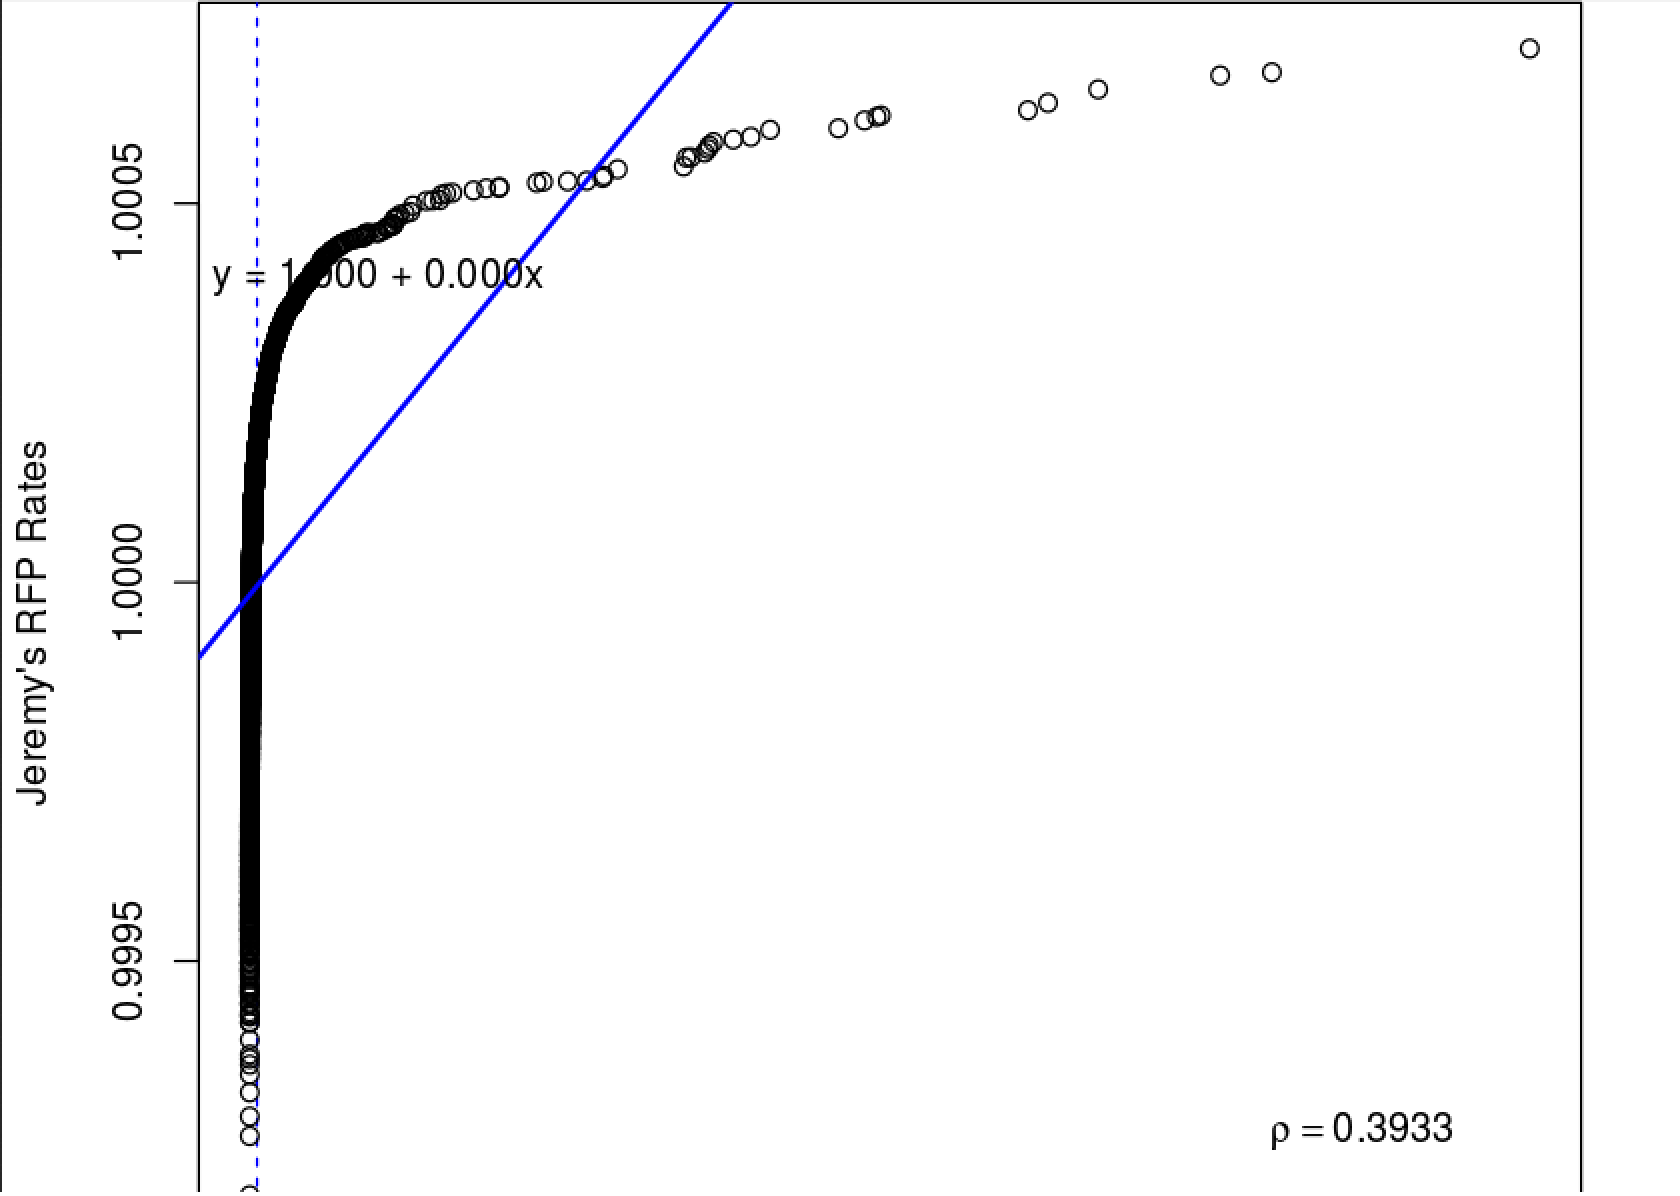
\includegraphics[width=\textwidth,keepaspectratio]{figures/7-27-16-JeremyCorrelation.png}
        \label{Jeremy Correlation 7-27-16}
    \end{figure}
    \item The bottom axis, not shown (see the file RFPJeremyConfidenceIntervalsForAlphaAndLambdaPrime.pdf, figure on the final page, under the folder 7\sep -\sep 27\sep -\sep 16\sep -\sep Jeremy\sep Correlation under the folder RunnableScriptsAndData/runLogs) is True Values.
        \footnote{mikeg: Please do not put incomplete figures and make sure all axes are well documented in the notebook.
        For example, what exactly are the RFP rates? The gene specific estimates of $\phi$? $\ln(\phi)$?  Don't assume you'll remember.
        Also please note that for a number of reasons, we generally visualize the log of expression, not expression itself.
}
        \footnote{Hollis: 08/03/16 -- Acknowledged and resolved in-person.
        They were the gene-specific estimates of $\phi$}
    \item I am not sure how to interpret this data. 
    While with 10 samples it had plotted a very nice x = Cy correlation as mentioned before, this data implies that the estimated values have a log relationship to the true values.
    \item May have to ask someone how to extract the Phi values -- perhaps the Trace chosen was wrong?
    \item In the meantime, simulating a genome to get data run another 20,000 samples on.
    \item I am basing my R script off of simulate\sep FONSE\sep .\sep R found in Rib\sep Model\sep Dev.
    \item The .fasta file we will use is \enquote{s288c.genome.fasta}, currently found in Rib\sep Model\sep Dev\sep /\sep data\sep /\sep real\sep Genomes.
    \item The LambdaPrime, Alpha, and Phi values can be recycled from Jeremy's folder, however.
    \item Talk with Dr. Gilchrist:
    \begin{itemize}
        \item Considering using code to include literal code text without needing to copy and paste the whole plaintext:
        \begin{lstlisting}
        Scripts/script_name.R

        \listinputlisting[language=R]{Scripts/script_name.R}
        \end{lstlisting}
        \item This would allow me to include and describe scripts to be put into this notes repo.
        \item Can also limit the number of lines printed: \enquote{language=R, firstline=2, lastline=12} (default is beginning and end of file).
        \item Can add captions (\enquote{caption=This is a caption}) to the same square bracket part.
        \item This caption would be displayed in a list of listings (\verb+lstlistoflistings+).
        \item The data looks weird and logarithmic because it's meant to be... use an option to make it log-log-based plotting, since the errors are log-distributed.
        \item Try adding in mean and variance waiting time ($\frac{\alpha}{\lambda\prime}$ and $\frac{\alpha}{\lambda\prime^2}$) to plot\sep .\sep Rcpp\sep \_\sep Trace (so under plot\sep Trace\sep Object\sep .\sep R).
        \item Ideally we'd plot confidence intervals on top of these plots, but the code for how to do this is unknown.
        See upper\sep .\sep panel\sep .\sep plot with its sd.x and sd.y arguments.
        The information should be there with how to calculate mean, but it isn't, so ignore this for now.
    \end{itemize}
    \item Rebased my local labnotebooks to clean up excess output files being included (and commit history).
    \item Next step: Plot with log-log in mind Phi, Alpha, Lambda, and Mean and Variance Waiting Time the data I already have from the Jeremy Simulated Genome run.
    \item Therefore, first let's implement mean and variance waiting time in the overall package.
    \item Looking at the code, we do calculate the posterior mean for Alpha and Lambda.
    Perhaps use this in place of taking the final element of the trace.
\end{itemize}

\labday {July 28, 2016}

\begin{itemize}
    \item Because of the difficulty and confusion from graphing these parameters and the fact that we don't want to re-invent the wheel, I took a pause from actually scripting to document some of these functions.
    \item TODO: Ask Cedric if it's better to implement waiting time functions in R (like I've done already) or in C.
    \begin{itemize}
        \item Asked on July 29, 2016 -- My current implementation is fine.
        I should consider renaming it to something better, but Cedric doesn't have any ideas currently either.
    \end{itemize}
\end{itemize}

\labday {July 29, 2016}

\begin{itemize}
    \item Continuing to try to figure out how to plot these functions properly.
    \item Specifically, Cedric mentioned yesterday that there were some functions that already plotted the mean of some parameters, and I should try to find the code and modify it as needed.
    \item Unfortunately, plotParameterObject only plots Mutation and Selection for the ROC and FONSE models, with only a TODO note listed for RFP.
    \item TODO: Ask Cedric where best to implement RFP functions in the existing functions in the package.
    \begin{itemize}
        \item It seems fine to just expand as I go from where existing TODOs have been posted.
    \end{itemize}
    \item Getting tired of scanning functions without documentation trying to figure out how to implement these functions.
    Going to return to trying to simulate a genome and running the simulation, I will plot the data afterward.
    \item Chat with Dr. Gilchrist:
    \begin{itemize}
        \item It should be easy to convert existing code to plot in the package from ROC to FONSE/RFP, but it hasn't been.
        \item Re-explained the problem: while getting the whole trace plotting was simple to extend (as I have done by adding mean and var waiting time), the existing code to get the codon specific posterior mean was in a function (getCSPEstimates) that was to be used specifically for ROC.
            \footnote{mikeg: 08/03/16 -- I can't find this function in the RibModelFramework repository using the command \enquote{grep -r \enquote{getCSPEstimates}}.
            You should be more clear in identifying files and functions.}
            \footnote{Hollis: 08/04/16 -- Using that same command in the top level of the repository yields the function under RibModelFramework/R/parameterObject.R. 
            Resolved in-person.}
        \item There was even a TODO note to implement this function in a variation for FONSE and RFP.
        \item Suggestion by Dr. Gilchrist: avoid \enquote{copying and pasting} code and reproducing it, rather find a way to make it easily extendible like the existing trace plotting has been.
        \item Would have to talk to Cedric about this.
    \end{itemize}
    \item In the process of writing an R script to simulate the genome, I finally found Gabriel's script to simulate the genome.
    He had written it in the main of the main package (thus, in C++).
    Since my script was already almost done, however, I decided to keep my work.
    Since it is written as an R script instead of inside of main like Gabriel had done, I can more easily save this script, not to mention document it so other people can find it again.
    \item Unfortunately, this script crashes in R with no error messages once it tries to simulateGenome.
    The one change I really did compared to the simulateFONSE.R was expose simulateGenome for RFP in R -- both ROC and FONSE already have (working) exposed functions to simulate genomes.
    Decided for the sake of running an overnight simulation to just copy Gabriel's C-side code anyway.
    \item TODO: Debug this. 
    This simulateGenome function is otherwise useless for most people -- they should not have to write C++ code to use it, and without it in R the R-side code would be redundant.
    \lstinputlisting[language=R, firstline=2, caption="Script to simulate an RFP-based genome."]{../RunnableScriptsAndData/scripts/simulateRFP.R}
    \item Running simulateGenome (with RFP) in C++ works fine, but our implementation of writing RFP files does not preserve the number of codons -- this is intended, as only the RFP\_Counts is important.
    Thus, the resulting file -- \enquote{HollisSimulatedGenome.csv} -- has \enquote{NA} for each Codon\_Counts of a Codon.
    \item Chat with Cedric:
    \begin{itemize}
        \item To implement getCSPEstimates for RFP (since this is currently unimplemented except in ROC), would have to change at least a bit of the code, confirming that it was more difficult than a quick fix.
        \item RFP does not concern itself with AA's directly, but can work with the group list via getGroupList instead.
        \item Another implementation possibility: Implement an additional function variation of getting codon specific posterior means that will take in the whole vector of codons rather than one codon at a time.
        \item When getCSPEstimates was originally written, Cedric had known it would be (and it is, currently) extendible to FONSE.
        However, it is not currently extendible to RFP.
        \item This led to the TODO note about copying this function and adapting it to RFP, but now it may be simpler to make it generic as Dr. Gilchrist had suggested.
        \item To do so, change it from the suffix Rcpp\sep \_\sep ROC\sep Parameter to simply Rcpp\sep \_\sep Parameter or move this function completely underneath its parent function and avoid another wrapper.
        \item Note that in R code, the current implementation reflects object orientation and inheritance.
        Thus, it's probably better to change it to simply Parameter rather than wiping out the parent wrapping.
        \item Also, the crashing for simulateGenome points to a likely segmentation fault.
        I should try to run Rstudio with simulateGenome on the gauley server, or ask Alan to run it on Windows and Visual Studio when he's back -- both runs will have better error messages to help with debugging.
    \end{itemize}
    \item Re-running simulateGenome with the same file Gabriel used to simulate his genome (an RFP file) -- it is currently found as \enquote{HollisSimulatedGenome2.csv}.
    \item Finished the day by running with 20,000 samples only the second simulated genome using the same script used to run Jeremy's simulated genome, using 8 cores.
\end{itemize}

\labday{August 1, 2016}

\begin{itemize}
    \item Ran into problems reauthenticating into git, wasting some time fixing this.
    \item Began running with 20,000 samples the first simulated genome I had created last Friday, using 8 cores again on the same script.
    \item Again, while I have the data for now two different runs over 40,000 total samples, I need to implement graphing functions to display this.
    Started writing them today.
\end{itemize}

\labday{August 2, 2016}

\begin{itemize}
    \item Checked on the simulation that used the first genome I simulated: it was still running.
    \item According to the log file of the second genome I simulated, the run should last about 25.6 hours.
    Will have to wait for completion before I can do anything else with Gauley.
    \item Note: The run with Jeremy's simulated genome took only 20 hours.
    \item Continued trying to write functions to plot the data I have.
    \item Also sent over the simulateGenome script to Alan so he can help debug that function.
    \begin{itemize}
        \item Results inconclusive once Alan finally fixed his github problems.
        His script also crashes without any error messages printed.
        \item One idea Alan pointed out was that intializing the parameter object was significantly faster with my RFP script than it was with the similar FONSE script, despite the FONSE script using a genome file that was significantly larger.
        Perhaps I need to check if there is a bug with initialization with the Alpha and Lambda files.
        \item If anything, the bug should be in the section of R-code is encapsulated by the C code.
        \item Will test on Gauley next as runs will have finished by then.
    \end{itemize}
    \item To modify parameterObject.R with the ability to extract CSP posterior means and quantiles for Alpha and Lambda Prime, I needed to expose CodonsToAA from sequenceSummary.
    \item After doing so, I discovered that the function I was modifying had not been used in one of the older development scripts before.
    Thus, there may be a degree of uncertainty if it actually works.
\end{itemize}

\labday{August 3, 2016}

\begin{itemize}
    \item Yesterday's progress was stalled by a bug compiling the package: Need to update NAMESPACE.
    \item Finished naively editing our current file. TODO: Make this more easily modifiable by allowing us to use roxygen2 rather than manual edits.
    \item Talk with Dr. Gilchirst:
    \begin{itemize}
        \item Should try to let us add AAs rather than one-at-a-time codons to modifying RFP etc groupList parameter.
        I.E. currently there is no easy way to. Long-term TODO, low priority.
        \item Quickly hack up scripts to plot the data I have already.
        \item Just get, instead of just the tail of the trace, the last 20 items of the trace and average it. I.e. the posterior mean.
        \item What we want:
        \begin{itemize}
            \item Posterior Mean Lambda Estimate vs Lambda True
            \item Posterior Mean Alpha Estimate vs Alpha True
            \item Posterior Mean log(Phi) Estimate vs log(Phi) Estimate
        \end{itemize}
        \item Run these things until it reaches stationary section near the end.
        \item Just look at the existing scripts to see examples of restart file loading usage.
    \end{itemize}
    \item Debugging RFP's version of simulateGenome further:
    \begin{itemize}
        \item Unfortunately, cannot run on Rstudio server at all.
        May have to ask Cedric what the command is to locally reload the package on the server, if possible.
        \item Running a script directly on gauley: Error seems to be when the Parameter::getSelectionCategory is called, resulting in a SEGSEV or seg fault error.
    \end{itemize}
    \item More function generalization: Need to discuss plotModel.R with Cedric.
    \item Currently this file has two functions (plotting synthesis rates for ROC and FONSE) with identitical code.
    \item Perhaps generalize it for just models in general and then adding RFP functionality from there.
    \item In general, R code is still extremely fragmented and incomplete, particularly for RFP.
    \item One nice-looking function hierarchy to discuss in particular is found in plotParameterObject.R.
    \item This file has specific plot calls for the Parameter object for ROC and FONSE, but these functions just call a more general function (plotParameterObject).
\end{itemize}

\labday{August 4, 2016}

\begin{itemize}
    \item Had to fix some quirks with LaTeX, and later merge conflicts with git's labnotebooks directory.
    \item Contiuing to write code to plot the data I've gotten:
    \item TODO: Ask about Psi vs Phi. 
    It sees like this script that I've been modifying, and possibly many more, use Psi instead of Phi when referring to synthesis rate.
    \item Still having problems plotting the Alpha and Lambda Prime posterior means.
    \item The log(Phi) posterior mean has been for quite a while, so I may just plot those now until I can finally decipher why the R code doesn't work.
\end{itemize}

\labday{August 5, 2016}

\begin{itemize}
    \item Goal for today is to figure out restart files and just plot log-log Phi posterior means, and then continue to struggle with figuring out why the Alpha and Lambda Prime script part doesn't work.
    \item Reorganized notes again: Now separated between notes and figures, and runnable scripts and data.
    \item Cedric answer: Would probably prefer using plotModel.R's inheritance hierarchy.
    \item Cedric comment: For getCodonSpecificPosteriorMean to simplify R-side code, perhaps make it so that instead of returning one value at a time return an entire vector and avoiding an R-side for loop.
    \item In the course of messing with restart files, I can tell the following:
    \begin{itemize}
        \item To start an MCMC run again from a certain point in a prior set of runs, load a restart file into the parameter initialization rather than starting conditions.
        \item Restart files are saved every 10 steps, and only one is needed to reinitialize.
        \item To load the MCMC and the Parameter info for \textbf{graphing}, we must use the loadMCMCObject and loadParameterObject functions.
    \end{itemize}
    \item Playing with these functions, loading the saved .Rdat files seems to work perfectly: the .csv files re-produced are identical to the ones saved prior to this repository.
    \item One caveat that caused problems when re-loading the data is ensuring that the calculated plots are the same.
    \item In the scripts I used to run with 20,000 samples with the MCMC, I only changed one value -- the initial percentage of the trace for only one plot.
    \item In the new script I wrote to get a log-log plot of the estimated versus true Phi posterior means, I finally figured out where else this value must be changed to affect other plots.
    \item Thus, while the scripts took the last 30\% of the trace for one plot, they took the last 50\% of the trace for every other plot; my new plotting script will keep this consistent.
    \item For future runs and plots, a new variable has been declared to be stored as the percentage of the trace to take throughout the plots.
    \item Happily, there is a good correlation between Jeremy's estimated Phi values versus the true values.
    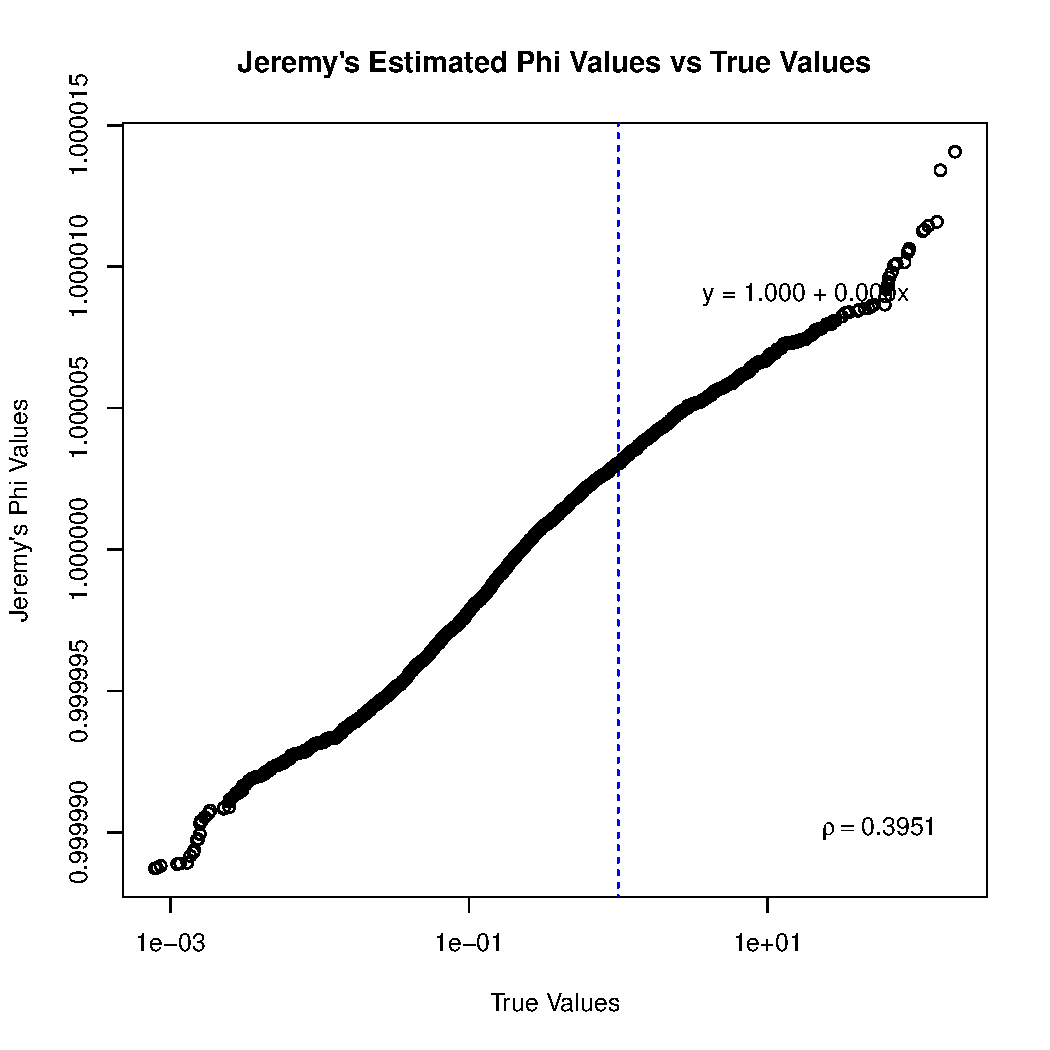
\includepdf[pages={1}]{../RunnableScriptsAndData/runLogs/7-27-16-JeremyCorrelation/newPDFs/RFPJeremyEstimatedVsTrue.pdf}
    \item This pdf file is \enquote{RFP\sep Jeremy\sep Estimated\sep Vs\sep True\sep .\sep pdf}.
    \item These new pdfs (the relevant page already included above) are found in Runnable\sep Scripts\sep And\sep Data\sep /\sep run\sep Logs\sep /\sep 7-27-16\sep -\sep Jeremy\sep Correlation\sep /\sep new\sep PDFs.
    \item Ending the day waiting for gauley's Rstudio console to stop spitting out error messages and clogging the system.
    \item Seems to be a bug with my quick edit to the ploting script to script with my own simulated genomes.
\end{itemize}

\labday{August 7, 2016}

\begin{itemize}
    \item Mostly worked with checking R-side functions today.
    \item Spent a lot of time looking up differences between R-side data structures, no real progress made however.
    \item TODO: Continue debugging scripts on Monday.
    Might have to bother Cedric at this point on how to write these scripts.
\end{itemize}

\labday{August 8, 2016}

\begin{itemize}
    \item Looking at gauley results: The outputted .pdf files from the error messages are, as expected, bugged.
    \item Not only are Lambda and Alpha Prime still bugged, but the plot for Phi values do not show up at all.
    \item Now rerunning the script line-by-line to find where the errors start happening.
    \item The error messages appear in a for loop that should work fine; error message is that indexes are out of bounds.
    \item Specifically, the parameter function call below spits out the error message:
    \begin{lstlisting}
    for (geneIndex in 1:length(genome))
    {
        psiList[geneIndex] <- 
        parameter$getSynthesisRatePosteriorMeanByMixtureElementForGene(
        samples * percentTraceIgnore, 
        geneIndex, 1)

        g <- genome$getGeneByIndex(geneIndex, F)
        ids[geneIndex] <- g$id
        //$ For latex syntax coloring fix only
    }
    \end{lstlisting}
    \item Initializing the second genome that I generated also crashes Rstudio for some reason.
    \item Restarted gauley Rstudio after a long delay and reran the script I used to produce the Jeremy pdf to export to labnotebooks, to compare the difference between this working script and the failing one for my own Genome.
    \item The script can now be found in RunnableScriptsAndData/scripts.
    \item This script will not work in labnotebooks because it requests several files located in different folders and more importantly requests giant .Rdat files that cannot be included in our git repo.
\end{itemize}

\labday{August 9, 2016}

\begin{itemize}
    \item Talk with Dr. Gilchrist:
    \begin{itemize}
        \item For R/initializeGenomeObject, default should be fasta.
        In retrospect looking at the code, this is already the default.
        \item Check at what gene the reading in drops out at for HollisSimulatedGenome.csv
        \item Comparing printed RFP file to read-in RFP file: identical. Dead end.
        \item Check the restart file's genes!
        \item RFPROC reading and writing RFP files may be completely wrong: We \textbf{need} the codon\_counts, but currently we do not preserve it.
        \item Recall Pop et al data (originally): Name, Length, Sum mRNA, Sum FP, FP per Codon, which is a mess.
        \item This data was simplified via Dr. Gilchrist's Mathematica script into the current RFPROC format.
        \item RFPROC: Format should be ID, RFP Count, Codon Count, Codon (current format).
        \item The NAs for codon counts that are not preserved \textbf{should} be filled in 
        \item When using Simulate Genome, all that should change out of this format is the RFP Count (compared to what was read in originally)
        \item This is, of course, since we are just making fake data as a simulation.
        \item PANSE: Format will be ID, RFP Count, Position, Codon
        \item For RFP Codon counts: Perhaps worry about ambiguous or non-observable positions.
        To do this, should be fairly trivia: let Position be an integer, with -1 meaning that this data should be discarded while other values are valid.
        \item New function: ProcessLareau: Should be pretty simple, let this be the default for now?
        \item TODO LATER: SimulatePANSE: just for each position, make RFP count number.
        \item TODO: Later on do Process Pop (which would also call readFasta) to get the RFPROC format or the PANSE format.
        \item On average, 61 calculations per gene for RFPROC/PA, 400ish per gene for PANSE since it's a per-position basis rather than a summary.
        \item FOR NOW, let's try and make the PANSE format the default and summarize it for RFP, rather than the current RFP being the default.
        \item Make RFP\_count data to have both long and short categories and combined.
        \item Gilchrist clarification: Don't make a combined category in C++ yourself.
        If the researcher wanted to have a combined category, they would have made it one of the categories like long and short, so simply treat is as another category to process.
        \item Make an integer defaulting to just calculating long category.
    \end{itemize}
    \item Modified an existing Perl script to now simply transform Lareau data to the new PANSE format.
    Script is now found in Runnable\sep Scripts\sep And\sep Data\sep /\sep scripts as \enquote{to\sep CSV\sep .\sep pl}.
    \item Also removed \enquote{plotRFPJeremy.R}, as it is redundant with \enquote{testJeremyRestart.R} (older version of same script function).
    \item PANSE format mentioned above was out-of-order.
    Format is geneID, position, codon, RFPcount[0] etc, as additional categories will be appended at the end.
    \item TODO: Rename the RFP model to PAModel to be similar to PANSEModel.
    Will also help solve confusion and needing to distinguish it as RFPROC.
    \item Next step is a longer process: Modify the function readPANSE (now readPA) to read in multiple different categories.
    \item First step is modifying the sequenceSummary data structure to allow for multiple categories: convert from vector to vector of vectors (one vector per RFP\_count category).
    \item Not committing current changes: Fails Unit Testing on Genome.cpp and reading in the new file format with the multiple category architecture (even though right now it's supposed to default to just one category).
\end{itemize}

\labday {August 10, 2016}

\begin{itemize}
    \item Pinpointed error from yesterday: It seems that when a Gene is retrieved from a genome, it does not retain the RFP\_count data in the new format.
    \item The functions themselves work perfectly, but something is lost when a gene with a vector of vectors representing RFP\_count for each category is added to a Genome.
    \item Once a Gene is added to a Genome, retrieving the Gene from the Genome results in a Gene with all the old data preserved, but not the new RFP\_count information at all.
    \item Commenting out existing functions revealed that when SequenceSummary::clear() is called, it clears RFP\_count, and somehow the new RFP\_count vector of vectors is completely cleared rather than once per gene.
\end{itemize}

\labday {August 11, 2016}

\begin{itemize}
    \item Continuing to try to figure out why the new RFP\_count structure is failing.
    \item Important note for future researchers: As of present, we have two different structures to count RFP data.
    \begin{itemize}
        \item RFP\_count is the currently-unused-outside-of-testing structure that is intended to be used for the PANSE model.
        It is currently going to be adapted to use for both the PA and the PANSE models.
        Also, I still haven't renamed the RFP model to the PA model yet.
        \item RFPObserved is the currently-used structure to record RFP data for the RFP model.
        Because the RFP model does not use a fasta file or anything else to record the number of codons, this may be incorrectly implemented.
    \end{itemize}
    \item Narrowing down bug location: SequenceSummary's clear() function is only called when a constructor is used OR when Gene::setSequence is called.
    \item The sequence summary constructor is implicitly called when a Gene object is constructed.
    \item Genome::addGene() does not create a Gene object, but Genome::getGene does:
    \begin{lstlisting}
Gene& Genome::getGene(std::string id, bool simulated)
{
	Gene tempGene;
	unsigned geneIndex;

	for (geneIndex = 0; geneIndex < getGenomeSize(); geneIndex++)
	{
		tempGene = simulated ? simulatedGenes[geneIndex] : genes[geneIndex];

		if (tempGene.getId().compare(id) == 0) break;
	}
	return simulated ? simulatedGenes[geneIndex] : genes[geneIndex];
}
    \end{lstlisting}
	\item In the next hour of work, I discovered that Gene::setSequence does clear the sequence summary.
	\item This is an intended feature of the function, but my implementation of reading in the PA file initialized the sequence summary's RFP\_count before setSequence is called, resulting in no initialization of RFP\_count (as it is cleared right after).
	\item This explains the bug I had been experiencing when I get the gene back out of the genome structure and tried to look at the RFP\_count data, which was lost (and resulted in a memory error).
	\item Normally, this error would be detected much earlier -- I had tried (and successfully did) print RFP\_count data before adding the gene to the genome.
	Under normal conditions, this indicates that the sequence had not been cleared and everything was fine until it was added to the genome.
	\item I suspect it was simply a lucky memory location that kept the RFP\_count data in the same place despite it being cleared, and when this retrieval call was done again on a copied gene, it called a different (non-existent) memory location.
	\item Thus, I fixed the problem that had delayed me for two days now by initializing the RFP\_count data after setting the sequence.
\footnote{mg:Strong argument for \emph{always} initializing your structures, at least during code development.
Would have saved you 2 days of work.
Ahh the school of hard knocks.
}
\footnote{Hollis: 08/23/16 -- Noted! See August 23 notes -- we're probably going to just make this function a part of a constructor to (mostly, hopefully) guarantee a size is assigned rather than assuming there are no categories.}
	Also added more notes on this effect, since it was documented before but not as emphasized.
	\item New format passed tests; now to use these new categories rather than defaulting to just one.
\end{itemize}

\labday {August 12, 2016}

\begin{itemize}
    \item Currently continuing debugging from yesterday -- reading in with multiple categories currently results in exit code 6, which Google says is a SIGABRT signal.
    \item This error occurs sporadically in the code, which makes me think this is another (difficult to solve by nature) memory error; there is no consistent place where it occurs, but I suspect it is in the reading of the PA file format.
    \item Further testing with code practically confirms a memory error: same code has different results when run, one time passing and another time failing.
\footnote{mg:Nice job testing this hypothesis.}
    \item These errors are difficult to check on Mac (hence the time spent debugging); may need to ask Alan to run Visual Studio debugger etc which are available on Windows.
	\item To account for possible bugs with multiple categories, limited it back to a single category but with the new code to read in with multiple categories possible.
    \item A snippet of code I'm running to check the differences between genomes being read in (panse) versus the hard-coded Unit Testing data (testGenome):
    \begin{lstlisting}
     	Gene blah1 = testGenome.getGene("TEST001");
        Gene blah2 = testGenome.getGene("TEST002");
        Gene blah3 = genome.getGene("TEST001");
        Gene blah4 = genome.getGene("TEST002");
        std::vector <unsigned> blah1Vect = blah1.getRFP_count(0);
        std::vector <unsigned> blah2Vect = blah2.getRFP_count(0);
        std::vector <unsigned> blah3Vect = blah3.getRFP_count(0);
        std::vector <unsigned> blah4Vect = blah4.getRFP_count(0);

        my_print("testGenome gene 1: size %: ", blah1Vect.size());
        for (unsigned i = 0; i < blah1Vect.size(); i++){
            my_print("% ", blah1Vect[i]);
        }
        my_print("\ntestGenome gene 2: size %: ", blah2Vect.size());
        for (unsigned i = 0; i < blah2Vect.size(); i++){
            my_print("% ", blah2Vect[i]);
        }
        my_print("\npanse gene 1: size %: ", blah3Vect.size());
        for (unsigned i = 0; i < blah3Vect.size(); i++){
            my_print("% ", blah3Vect[i]);
        }
        my_print("\npanse gene 2: size %: ", blah4Vect.size());
        for (unsigned i = 0; i < blah4Vect.size(); i++){
            my_print("% ", blah4Vect[i]);
        }
	\end{lstlisting}
	\item The outputs vary wildly, always with a difference between the last gene's RFP\sep \_\sep counts.
	\begin{lstlisting}
testGenome gene 1: size 4: 0 2 0 0 
testGenome gene 2: size 4: 0 0 1 1 
panse gene 1: size 4: 0 2 0 0 
panse gene 2: size 4: 2 0 0 0 
	\end{lstlisting}
	\begin{lstlisting}
testGenome gene 1: size 4: 0 2 0 0 
testGenome gene 2: size 4: 0 0 1 1 
panse gene 1: size 4: 0 2 0 0 
panse gene 2: size 4: 0 2684354560 3549298901 4026533884 
	\end{lstlisting}
	\item With this testing code reveal, fixed the error: It was related to the change in RFP\_count format yet again.
	\item I was clearing the entire vector of vectors, destroying the initialized structure that had the number of categories.
	Fixed by making it clear each vector inside of the vector of vectors instead.
	\item With this fixed, the package passes unit testing with multiple categories of RFP\sep \_\sep counts!
\footnote{mg: Yea!}
	\item Next step: Summarize this read in PA-format data into RFP summary data.
	\item Data to be summarized: RFP\_Counts and Codon\_Counts for each same Codon.
	\item Right now, RFP\_count data is stored as a vector ordered by the order in which lines are read in.
	\item Once again, this vector is encapsulated by a sort of summary vector to account for the different categories.
	\item Meanwhile, the other gene data is read in with the same format as other file formats, storing information as genes with sequence summaries and IDs but not preserving positioned RFPs.
	\item Need to think of a way to store this summary data.
	\item Also began to add support to ignore a line if its position is ambiguous (marked by integer -1).
\end{itemize}

\labday {August 16, 2016}

\begin{itemize}
    \item Our old data for PA files was in the form of Codons,Position rather than Position,Codons; changed this for ease of calculating what lines to discard (if position was unknown or ambiguous).
    \item Finished support for ignoring ambiguous lines, and added an example of this to unit testing.
\end{itemize}

\labday {August 17, 2016}

\begin{itemize}
    \item Now need to store position and count the number of times a codon occurs per gene.
    \item This would probably be stored in the Gene structure (while the RFP\_counts information was stored in the SequenceSummary structure).
\end{itemize}

\labday {August 18 - 19, 2016}

\begin{itemize}
    \item This labday set is merged because August 18 was mostly testing the package.
    \item Problem revealed: Currently, while the Lareau data has scrambled rfp\_counts for each codon for each gene, this is not supported.
    \item This means that if Gene A has the codon AAA defined, and then it is redefined later (when it should merely append to the existing data), it destroys the old data.
    \item First step is to add the ability to store the data position based: right now, data is read is purely on the order in which data is read.
    \item Cedric had encountered a weird error that turned out to be local-only when installing the package, while I had some bugs related to the Travis CI admins messing with sudo privileges and causing the server to not install the package.
\end{itemize}

\labday {August 22 - 23, 2016}

\begin{itemize}
    \item August 22 -- sick day.
    Filled out hours and updated to current repos.
    \item August 23 -- Mostly a discussion day with Cedric on how to re-implement RFPModel (TODO: Still need to rename this to PAModel).
    \begin{itemize}
        \item TODO: Screenshot taken of board to be uploaded to notes here.
        The board currently has a summary of the data structures Cedric and I have figured out.
        \item Beginning of talk with Cedric: Confirmed that Gabriel (probably) messed up with Codon\_Count calculations, and thus would indeed require a major rework of RFPModel.
        \begin{itemize}
            \item Privately asked Gabriel about prior work, but he doesn't remember the justification he and Jeremy had made about this calculation.
        \end{itemize}
        \item Current PA file read-in is largely deficient of information-storing structures to easily calculate log likelihoods.
        \item Core problem: While my new vector of vectors for RFP\_counts for different categories was a good start, we need to associate directly the codon (or, for convenience, the codon id as an unsigned integer) with the position and with the RFP\_counts from there.
        Currently, my vector of vectors does not track the codon, as I was intending to associate this data indirectly with the stored sequence string to re-find the codon internally each time.
        \item Solution: While looping over the string is a bad idea, we can still keep my vector of vectors as long as another, 1-dimensional vector is created that associates the position with the codonID, since each position can (should, if my ambiguous position check still works after I finally edit the code) only hold one codon.
        \item These two data structures, combined, can be re-summarized into the current RFPModel data: A 2-dimensional vector that sums the RFP\_counts for each category for each gene ID, and retaining the nCodons 1-dimensional vector (but actually storing the right number rather than doing voodoo Hanas calculations).
        \item Another major problem: Current functions to set sequence don't really work for RFP\_count based data.
        \item Since PA data is presented line-by-line with the size of the sequence unknown, we should make a new function to process and set this sequence at the very end of a set of genes.
        \item Currently, a PA file has consecutive gene IDs, so we can assume that all gene-wise information is correctly clustered together until the next cluster shows up.
        \item Additional discussion topic: How to read in data so that it's all associated easily.
        \item Cedric suggested reading in a table-style vector of vectors: For each line, make this a vector that is pushed unto a vector that is sized to the number of csv columns of the file.
        \item Planned steps:
        \begin{itemize}
            \item Add the position vector and the sumRFPCount vector
            \item Modify the Genome.cpp function reading in PA files: Store each line as a table-style vector of vectors
            \item Make sure to retain the current set-up of reading in the file twice, the first pass checking the size of the genome and each gene
            \item Then read in this vector of vectors in a function in Gene.cpp, a new version of setSequence that accepts a vector of vectors as an argument.
            \item This will concatenate each inner vector's sequence string together to form a sequence, etc.
            \item From the new setSequence, call processRFP in SequenceSummary.cpp: Accept a 2-dimensional vector, that same table, to finally store this information as well as summarize it.
        \end{itemize}
    \end{itemize}
\end{itemize}

\labday{August 24, 2016}

\begin{itemize}
    \item Began implementing plan set forth yesterday.
    \item Started by modifying (and thus simplifying, for now) the readPAFile function in Genome.cpp and added barebone support for setPASequence in Gene.cpp.
    \item TODO: Ask Cedric about SequenceSummary and the difference between codonArray and codonArrayParameter as required by the boolean forParamVector when using the function indexToCodon
    \item Current workload:
    \begin{itemize}
        \item Clean up defunct notes
        \item Continue cleaning up old, now defunct code to fit the plan
        \item NOTE (and note elsewhere and likewise fix defunct notes) that we don't need to read in the file twice anymore because the ingenious table design lets us extract the size of the gene from the number of rows of the table
        \item Currently code is a mess but works up to the point where it calls processPA: It reads in a PA file, ignores ambiguous positions still, but reads in the sequence correctly (and just the sequence, no internal storage of RFP data yet).
    \end{itemize}
\end{itemize}

\labday{August 26, 2016}

\begin{itemize}
    \item First step today: Construct the sequence position-based.
    Right now the sequence is read in based solely on file read-in order, ignoring position.
    \item Positioning was easily fixed thanks to using the new table format.
    \item Next: started writing processPA.
    \item Finished skeleton for processPA such that it runs and stores the data that is usually stored, but still need to implement new data structures.
\end{itemize}

\labday{August 29, 2016}

\begin{itemize}
    \item Began creating new data structures.
    \item While memory problems caused another small delay, finished creating and setting the data structures.
    \item TODO: Add helper functions to initialize, get, set, and in general check these data structures.
\end{itemize}

\labday{August 30 - 31, 2016}

\begin{itemize}
    \item August 30 -- Mostly was in the lab to discuss issues with other researchers.
    Did not actively work on own project.
    \item August 31 -- Recall: about half a month ago, Cedric asked me to fix getGenomeForGeneIndicesR, which was incorrectly implemented.
    \begin{itemize}
        \item I fixed the implementation, but did not have a chance to go back and unit test or error-check my changes.
    \end{itemize}
    \item Today Alex brought up a segmentation fault (memory error he was experiencing) after finally bringing all repositories up to date.
    Summary of problems and testing:
    \begin{itemize}
        \item On Gauley with R studio (running Gauley locally rather than remotely):
        \begin{lstlisting}
        *** caught segfault ***
        address 0xfffffffffffffff8, cause 'memory not mapped'

        Traceback:
         1: .External(list(name = "CppMethod__invoke_notvoid", address = <pointer: 0x2cdce60>,     dll = list(name = "Rcpp", path = "/usr/lib/R/site-library/Rcpp/libs/Rcpp.so",         dynamicLookup = TRUE, handle = <pointer: 0x2df0a00>,         info = <pointer: 0x7f3a5ebf9860>), numParameters = -1L),     <pointer: 0x238f690>, <pointer: 0x23a9af0>, .pointer, ...)
          2: genome$getGenomeForGeneIndices(genes.in.mixture, simulated)
           3: plot.Rcpp_ROCModel(model, genome, samples = samples * 0.1, mixture = 1,     main = "E.coli Codon Usage Plot")
            4: plot(model, genome, samples = samples * 0.1, mixture = 1, main = "E.coli Codon Usage Plot")
        //$ For latex syntax coloring fix only
        \end{lstlisting}
        \item For now, script and data file is located in \enquote{AlexTesting} folder under RunnableScriptsAndData, and can be run from scratch.
        \item Locally on his own machine (Ubuntu 15.2), he does not encounter any problems.
        \item This same script on my machine, however, runs into a memory problem as well:
        \begin{lstlisting}
          rsession(99676,0x7fff770b0000) malloc: *** mach_vm_map(size=4795577582035439616) failed (error code=3)
          *** error: can't allocate region
          *** set a breakpoint in malloc_error_break to debug
          Error: std::bad_alloc
        \end{lstlisting}
        \item Furthermore, both memory issues with error messages may occasionally run to crash R studio without any error messages at all.
        \item Currently, we suspect it is a machine or system-dependent bug.
        \item TODO: Ask Alan to run this script on windows because, once again, Mac lacks the memory-breakdown tools that Windows does.
        \item Also should reexamine the C++ code I wrote, just in case it is the problem.
        However, this is less likely (since once again, Alex's machine runs this without memory problems).
    \end{itemize}
\end{itemize}

\labday{September 2, 2016}

\begin{itemize}
    \item I want to prioritize looking at getGenomeForGeneIndices.
    \item I haven't set up a separate development branch from my own repo, so while I could look up Cedric's main repo I cannot push any major edits.
    \item Since Alex isn't in today either, I'm going to try and polish off the PA file reading and then finally push these changes to the main repository.
    \item Finished adding helper functions for sumRFP\_count information.
    \item The unit tests for everything with RFP\_counts now works again after changing the data structure style of RFP\_counts, and RFP\_counts testing takes into account position (and is position-based from index 0 to index n).
    \item TODO: Test the helper functions for sumRFP\_count work.
    \item TODO: Add a checker to ensure all the positions are correct for my new positionCodonID vector.
    \item TODO: Of course, remove the old RFPObserved structure and edit the code so that it not longer uses this miscalculation.
\end{itemize}

\labday{September 8, 2016}

\begin{itemize}
    \item Mostly discussion with Cedric about the contents of the email Dr. Gilchrist sent on September 7, 2016.
    \item The following have been copied from my quickly jotted notes:
    \item \enquote{Same weird stuff that Cedric mentioned with genome\$read\sep Observed\sep Phi\sep Values, where it somehow enters the error loop and starts setting things when it shouldn’t in byID}
    \item \enquote{Also seg faults inconsistently (memory error somewhere in this function)}
    \item \enquote{Restart files: Can be put as an argument into parameterObject. Should make it more clear that this argument is a restart file initialization. Maybe rename as "initWithRestartFile" instead of just "restartFile"}
\end{itemize}

\labday{September 12, 2016}

\begin{itemize}
    \item Sporadic work done over the last week.
    Mostly discussion-related, nothing concrete to report.
    \item Alex seems to have nailed down the error: getGenomeForGeneIndices takes a R-style vector (1-indexed) while it uses C++ code that is 0-indexed.
    \item He should have fixed it, but Cedric as of today (September 11, 2016) is asking for help to check why this new function is failing the Unit Checks (I had thought that they didn't even check this function)
    \item Checking this code with my fresh repo without committed changes (still a major TODO; school work has set me behind): I also get a failure in unit testing.
    \begin{lstlisting}
* checking tests ...
  Running 'testthat.R'
 ERROR
Running the tests in 'tests/testthat.R' failed.
Last 13 lines of output:
  Error in Genome::getGenomeForGeneIndices. An index specified is out of bounds for the genome!Returning empty Genome.Error in Genome::getGenomeForGeneIndices. An index specified is out of bounds for the genome!Returning empty Genome.MCMCAlgorithm is/setEstimateSynthesisRate --- Pass
  MCMCAlgorithm is/setEstimateCodonSpecificParameter --- Pass
  MCMCAlgorithm is/setEstimateHyperParameter --- Pass
  MCMCAlgorithm is/setEstimateMixtureAssignment --- Pass
  ERROR: Cannot set steps - value must be smaller than samples times thinning (maxIterations)
  MCMCAlgorithm get/setStepsToAdapt --- Pass
  MCMCAlgorithm getLogLikelihoodTrace --- Pass
  Error in initializeMCMCObject(samples = samples, thinning = thinning,  : 
    unused argument (thinning = thinning)
  Calls: test_check ... source_file -> eval -> eval -> initializeMCMCObject
  testthat results ================================================================
  OK: 72 SKIPPED: 0 FAILED: 0
  Execution halted
    \end{lstlisting}
    \item Later in the day Cedric mentioned that the readObservedPhiValues bug mysteriously resolved itself.
    No idea what changed (nor does Cedric), but because of the mounting task load I'm shelfing that potential problem as well.
    \item Ended day by confirming that read\sep PA fully works putting in positions and RFP\sep \_\sep counts.
    \item Next TODO to finally push to main repo: test the newly implemented RFP data models, particularly a summation of each RFP\_count per index.
\end{itemize}

\labday{September 13, 2016}

\begin{itemize}
    \item After hardcoding in the unit testing for readPA for the RFP data models, I unfortunately encounted no change in testing results.
    \item Expected result was that, since I enabled checking sumRFP data structures, there should have been an error immediately.
    \item Whether or not I modify the hard-coded sumRFP that is checked versus the read-in genome, I get a successful check.
    \item Currently suspect that it's related to how I still haven't implemented unit testing for the smaller component getter/setter functions. This is my next step.
    \item Ended the day by writing the unit testing for the getter/setter functions, but the readPA weirdness still occurs.
    \item Looking things up, a simple == statement should check if C++ arrays are equivalent (or, more importantly, if they're not); not sure at the moment how to proceed debugging this.
    \item In the meantime, finally pushed notes.
\end{itemize}

\labday{September 15, 2016}

\begin{itemize}
    \item Mostly checked up with Dr. Gilchrist on progress.
    \item Very busy with classwork -- will take a break until after midterms.
    \item TODO: I should keep checking with these C++ arrays, especially since in terms of implementation they are as easy as vectors to use and they should be more efficient.
    \item Let's start with printing out each element of the arrays and make sure they're even properly constructed.
    \item Also want to see why it is that I \textbf{always} get a success even when I'm expecting a failure -- check on a smaller level with getter/setter functions.
\end{itemize}

\labday{September 26, 2016}

\begin{itemize}
    \item Finally back to working after taking a break due to classwork -- quick recap of things to do:
    \begin{itemize}
        \item First, check C++ arrays and ensure they're working.
        \item Then, finally push my changes -- very far behind in this instance of the package but should have no merge conflicts.
        \item New issue cropped up today as mentioned by Cedric: Investigate memory issues with R-side initialization of Parameter objects.
        \item It seems that the memory that is allocated is never properly deleted.
        \item We fixed some memory issues by changing copy constructors to pointers, so multiple instances should not be created -- still, need to see why it is that Parameter is never deleted when Model is deleted (despite Model calling delete Parameter).
        \item First step to that that I suggested was to simply make a loop in C++ to create and delete Parameters, Genomes, etc. and see if it ever memory leaks (it shouldn't).
    \end{itemize}
    \item Another thing to do next time I come back is to change many of my testing functions to also return pointers and references rather than copies of objects -- would likely save time when running tests.
    \item Biggest change: finally finished implementing readPA!
    \item Seems like the work I'd been doing slowly but steadily with unit testing revealed what I now think caused the constant successes: the == checks were not accounting for the new data strucutres.
    \item In addition to this, even when the == comparators did check the new data structures, memory oddities had occurred because my C++ arrays were not initialized -- this was fixed by calling fill(0) after creating each array.
    \item Latest change to finally fix and push the commit was to fix a hardcoding error / series of typos that made the unit testing fail.
\end{itemize}

\labday{October 12, 2016}

\begin{itemize}
    \item Getting back into work, hopefully consistently, now that school has lightened up a bit after Fall Break.
    \item Starting with checking Unit Testing: Currently, we have four failures.
    \begin{itemize}
        \item First three failures are the result of renaming logLikelihoodTrace to logPosteriorTrace on only the R-side code (some of it) without editing the existing Unit Testing files nor the cpp files.
        Renamed the two functions affected (get and set functions) to logPosteriorTrace.
        \item The final failure is somewhere in the cpp code's unit testing for testParameter.
        \item Error was in Testing.cpp.
        Cedric had changed one of the hard-coded values in the function being tested (initParameterSet) and the Unit Testing hadn't been edited accordingly.
    \end{itemize}
    \item With this change pushed, the framework passes existing Unit Testing again.
\end{itemize}

\labday{October 17, 2016}

\begin{itemize}
    \item Mostly reset my environment -- Cedric approved my change, and now I should plan the next steps.
    \item Talked with Dr. Gilchrist on October 13, 2016.
    \item Basically reviewed my progress on the PA-structure code.
    \item Ideally, the extension into PANSE should be based on existing RFP code that has been corrected.
    \item This code should have control flow such that if nonsense error is 0, it uses the \enquote{streamlined and efficient} RFP/PA code rather than the general PANSE code.
    \item I should rename the \enquote{RFPObserved} to the present RFP-containers.
\end{itemize}

\labday{October 28, 2016}

\begin{itemize}
    \item Slowly removing RFPObserved functions and variables.
    \item TODO: Figure out unified name for RFPCount (or RFP\_count).
    \item Work done as of today:
    \begin{itemize}
        \item Commented out RFPOBserved in Gene, SequenceSummary.
        \item Added getSumRFP\_count at a category for a codon string.
    \end{itemize}
\end{itemize}

\labday{November 18, 2016}

\begin{itemize}
    \item Standardized RFP\_count as RFPCount since other variable names with abbreviations, such as those with the abbreviation AA, are in this style (AAToAAIndex etc).
\end{itemize}

\labday{January 10, 2017}

\begin{itemize}
    \item Debugged a personal Mac issue with workflow speed: Newest update had messed up my SSH authentication, so I had to spend some time today just fixing this to return to usual work.
\end{itemize}

\labday{February - March 2017}

\begin{itemize}
    \item Let Cedric handle the Travis Hmisc error in the description.
    \item Make the writing function a priority! -- Finish by March 9th.
    \item Talked to Cedric later that day (March 1st) -- He knows about the Hmisc error but doesn't know how to fix it.
\end{itemize}

\labday{March 8th, 2017}

\begin{itemize}
    \item Chose to add an array of strings describing the names of the RFP count categories to Genome.h.
    \item Implemented positionCodonID detection into the functions.
    \item End of day result: Writing function 90\% completed writing function.
    \item Will comment out testing for now, return later.
    \item Currently my position vector only stores the codon ID, while RFP counts store the sum of the RFP for each category (or sum of all).
    \item Need to record RFP data for each position for each category -- I'm thinking another vector of vectors, outer vector being position and inner being a vector of RFP values.
\end{itemize}

\labday{March 9th, 2017}

\begin{itemize}
    \item Notes on Gilchrist meeting:
    \item OK'd spring break schedule: I will be away taking care of my health for Monday through Wednesday and return Thursday afternoon.
    \item TODO (after finishing writing function):
    \begin{itemize}
        \item Generate data.
        \item Use a wide range of values, ensure bugs are not being masked (edge cases).
        \item See if results are similar to what are expected.
        \item Fit real data, see if well-correlated.
    \end{itemize}
\end{itemize}

\labday{March 16, 2017}

\begin{itemize}
    \item Back in the office, decided to help with debugging Travis and R CMD check since Cedric was also in.
    \item Cedric will be gone tomorrow + next week, so I'll return to main work then.
    \item Added Hmisc to travis.yml -- this fixes Hmisc on my Travis check, pushing to main now when Cedric's ready.
    \item Added acf to imports for NAMESPACE.
    \item Used document() to update the documentation changes Cedric made.
\end{itemize}

\labday{March 17, 2017}

\begin{itemize}
    \item Finishing the writing function.
    \item Goal: need to record, for each position, the RFP values for each category. All other info is optional or already stored elsewhere.
\end{itemize}

\labday{May 16, 2017}

\begin{itemize}
    \item Returning to full-time work -- looks like I've missed a chance to submit a pull request on my work before the school semester had ended.
    \item I have some backlogged local changes I need to debug ASAP.
    \item There currently seems to be a bug in the writing function where I misdirect the writing output and overwrite the file I had originally read in.
    \item Fixed it as well as updated the testGene.R file to account for a new parameter, categoryIndex, in the updated function for getRFPObserved.
    \item Pushed a change that added and tested getSingleRFPCount (used in writing the PA file), a helper function called testGenomePAHelper for testing the PA file genome creation, and finalized and tested the writePA function.
    \item Spent some time resolving a ton of merge conflicts due to failure to update with the team during the semester.
    \item Requested a pull finally adding Hmisc, added c++ code for RFPCategoryName support, position-based storage of codon IDs, writePA, getSingleRFPCount.
\end{itemize}

\labday{May 17, 2017}

\begin{itemize}
    \item Will begin removing old code for readRFP format.
    \item Currently debugging errors from updating R from 3.3 to 3.4 -- may be related to the updated RibModel package using openMP, even on Mac which doesn't have openMP support.
\end{itemize}

\labday{May 18, 2017}

\begin{itemize}
    \item openMP flags that were added by Cedric don't currently check OS, but there's a way to fix that -- TODO, investigate makevars.in and a configure file to detect system OS to enable/disable openMP.
    \item Finished fixing R installation errors -- had to individually reload packages between versions, rather than blindly moving installed files.
    \item Decided to try and debug the Makevars issue between versions via using autoconf and configure.ac file.
\end{itemize}

\labday{May 22, 2017}

Agenda for today: Finalizing openMP issue, planning for tomorrow's simulation runs to test the RFP model again (TODO: Still need to rename it... Low priority).

\begin{itemize}
    \item Talked with Dr. Gilchrist and Brian about the openMP issue.
    \begin{itemize}
        \item Formerly, Cedric had the Makevars file attempt to use openMP if available -- this allowed the RibModel package to run out-of-the-box for all systems, but this code was not CRAN-compliant.
        \item On May 14, Cedric made Makevars CRAN-compliant by adding code according to the CRAN manual for writing Makevars files enabling openMP.
        \item This code works for Linux and Windows, but it does not work out-of-the-box for Mac.
        \item I had begun writing fairly complicate autoconfigure files and Makevars alternatives that detects the system in R, while installing the package, and more, but this seemed extraneous (code based on ARTP2 package in CRAN).
        \item Instead, asking Brian, it seems OK to leave the code like Cedric had -- it had passed on CRAN, after all. The basic idea is that it works on two of the three primary operating systems (Windows, Linux, but not Mac).
        \item Mac users must instead download their own solution to the lack of openMP as needed, and we will include a note in the DESCRIPTION file to address this need and link to help.
        \item For me and other researchers working on Mac, this can be easily accomplished by symbolically linking an openMP-enabled compiler on top of the under-supported Apple default.
        \item I will also write a much simpler configure file to detect the operating system and inform the user of the lack of openMP support.
        \item It should be noted that upon further investigation, CRAN allows the source files to have this openMP Makevars support, but it seems the binaries for OSX completely exclude this: see package mvnfast, which cannot be installed via source files but can via specific binaries.
    \end{itemize}
    \item Cedric's input is that the more complicated configure script is probably preferred, especially with the new information about the difference between the source and binary package of the other openMP example in CRAN.
    \item For now, I am pushing the simpler configure file that informs the user, on package installation failure, that the cause is the lack of openMP -- users will be slightly more able to install openMP as needed compared to before (when there would be a missing compiler flag).
\end{itemize}

\labday{May 23, 2017}

\begin{itemize}
    \item Finished modifying the more complex configure script to account for OSX.
    \item Now the Makevars file is dynamically created per package built to account for existence of openMP.
    \item While testing Makevars compatibility between systems, I tried to use both Gauley and Newton.
    \item Gauley seems to be having consistent issues with checking the update ribModel package. I will have to debug this later, for now I'll try to use Newton.
    \item Also setting up SSH permissions and keys to more easily use Newton and Gauley -- Newton can now be accessed via SSH, and both can use my github directory permissions.
\end{itemize}

\labday{May 24, 2017}

\begin{itemize}
    \item Returning to fix up and test RFP model. TODO ASAP out of annoyance: rename it already, I've mentioned renaming it for months.
    \item Note that Gauley still doesn't compile the package correctly; Newton, meanwhile, does.
    \item Tasks done:
    \begin{itemize}
        \item Removed old readRFP and writeRFP functions completely (they were commented out before).
        \item Fixed up some documentation around these areas of code.
        \item Cleaned up testing folder and naming convention. No longer using .pa convention, but .csv instead for universal standard.
        \item Removed desc folder since it is now in RibModelDev.
    \end{itemize}
\end{itemize}

\labday{May 26, 2017}

\begin{itemize}
    \item Renamed all instances of RFPModel, RFPParameter, and the like to PAModel, PAParameter, etc.
    \item TODO: Ask Cedric the standard format to write something in the DESCRIPTION file strongly suggesting a user have access to OpenMP, even though it's not longer necessary.
    \item Added a case for reading in PA data: If a codon count is < 0, it is assumed to be a typo, and 0 is input instead.
\end{itemize}

\labday{May 30, 2017}

\begin{itemize}
    \item Asked Cedric about the DESCRIPTION file explicitly mentioning openMP -- the other openMP-enabled CRAN module I reference (ARTP2) for our own configure file does not mention it, so he thinks we can ignore it as well.
    \item Gilchrist talk:
    \begin{itemize}
        \item Likelihood of an RFP count: With a negative codon count value, don't modify the likelihood at all.
        \item Rethink the \enquote{If a codon count is < 0, set to 0} idea from the May 26th notes. Instead, if an RFP count value is ambiguous or unknown, it can be set to -1 and ignored \textit{for just that category}. This is what is meant by it not affecting the Likelihood.
        \item From Dr. Gilchrist's board: if x(arrow) = {x1, x2, x3} and x(arrow prime) = {-1, x2, x3}, then LogLikelihood (xarrow) = summation of the Loglikelihood of each xi (three of them), and LogLikehood (x arrow prime) = summation of the Loglikelihood of each valid xi (two of them).
        \item In terms of implementation, store the line after all (keeping the RFP count at -1) but when calculating Likelihood, ignore that -1 (for example, setting it to 0 for Likelihood only).
        This would also make retaining data better when re-printing out information.
        \item Make sure the user can specify which category to use of the multiple we have stored (TODO, but obvious when/where!)
        \item For the record, \textbf{I have fixed the August 9th bug that was originally in RFP}. ncodons are correctly calculated. This was fixed when I split \enquote{processSequence} in sequenceSummary.cpp with PA's version, which is \enquote{processPa}.
        \item Also went over the Gauley check bug with Dr. Gilchrist (it was not a compilation error, but a check error; avoid that terminology confusion in notes). It seems the R code checks spitting out a ton of notes is just a \enquote{possible} problem and may not affect the actual package. Recall: There still is some weird random number seeding discrepancy between Gauley and other machines that results in the literal value checking of testMCMCROC to fail. This is fine; remove the check for Gauley-only.
        \item Meeting concluded with Dr. Gilchrist updating Gauley's version of R to 3.4. Will re-check the passage for bugs.
    \end{itemize}
    \item Next step is simulating a genome and compare with Pop's data.
\end{itemize}

\end{document}
